\documentclass[11pt]{article}

% ============================================================
% Packages
% ============================================================
\usepackage[utf8]{inputenc}
\usepackage[T1]{fontenc}
\usepackage{lmodern}
\usepackage{geometry}
\geometry{margin=1in}
\usepackage{amsmath,amssymb,amsfonts,amsthm}
\usepackage{booktabs}
\usepackage{longtable}
\usepackage{hyperref}
\usepackage{cleveref}
\usepackage{algorithm}
\usepackage{algorithmic}
\usepackage{tikz}
\usetikzlibrary{arrows.meta,positioning,fit,calc,decorations.pathreplacing,shadows}
\usepackage{caption}
\usepackage{enumitem}
\usepackage{xcolor}
\usepackage{microtype}
\usepackage{listings}
\lstdefinelanguage{Lean}{
  morekeywords={theorem,def,abbrev,inductive,structure,where,fun,Prop,Type,let,in},
  sensitive=true, morecomment=[l]{--}}
\lstset{language=Lean, basicstyle=\ttfamily\small\upshape, columns=fullflexible, keepspaces=true,
  mathescape=true, keywordstyle=\bfseries\upshape, commentstyle=\itshape\color{gray},
  xleftmargin=1em, aboveskip=4pt, belowskip=4pt}
\usepackage{stmaryrd}
\usepackage{natbib}
\usepackage{authblk}

\hypersetup{
    colorlinks=true,
    linkcolor=blue!70!black,
    citecolor=green!50!black,
    urlcolor=blue!70!black
}

% ============================================================
% Custom commands
% ============================================================
\newcommand{\gerundelle}{\textsc{Gerundelle}}
\newcommand{\sov}{\textsc{SOV}}
\newcommand{\leanus}{\textunderscore\allowbreak}
\newcommand{\lean}[1]{{\let\_\leanus\texttt{#1}}}
\newcommand{\R}{\mathbb{R}}

% Each guarantee is stated first in plain terms, matching its Lean statement. Its
% interpretation follows under "Reading", and the classical result it instantiates
% under "Prior work", kept separate on purpose.
\newtheorem{theorem}{Theorem}[section]
\theoremstyle{remark}
\newtheorem*{reading}{Reading}
\newtheorem*{prior}{Prior work}

\title{\textbf{GERUNDELLE: A Formally Verified Architecture of Mind} \\[0.5em]
\large Twelve Layers, from World Physics to Narrative, Machine-Checked in Lean~4}

\author{Scott Seto}
\affil{Independent Researcher}
\date{October 2026}

% ============================================================
\begin{document}
% ============================================================

\maketitle

% ============================================================
% ABSTRACT (rewrite v1)
% ============================================================

\begin{abstract}

Where should a mind's correctness live? In a neural network trained end to end, it lives in
behavior: the network is trained to keep the distinctions a mind must keep (between what it
saw and what it imagined, between what it lived through and what it was told), but nothing
guarantees that it does. Compartmentalization in neural networks is an open problem.
\gerundelle{} places them instead
in the mathematical structure of the mind's operators, where they can be stated exactly and
proved.

\textbf{\gerundelle{}} is a twelve-layer architecture of mind whose promises are theorems.
Its layers run from a world that conserves its one physical quantity, through perception,
competition for attention, provenance of evidence, memory, understanding and self-awareness,
to ownership, affect, planning, social exchange and the selection of what is worth telling.
Each layer carries guarantees that a proof assistant (Lean~4) has checked for every possible
input, every possible sequence of operations, every possible interleaving. The development
comprises \textbf{24 files}, \textbf{301 theorems}, and \textbf{no unfinished proofs}.

The architecture is domain-independent: one mind and one algebra run in story, code, chess
and population worlds, with no domain-specific machinery, and only the world changes. The
domains are projections, not separate systems. Because most of the guarantees are stated
over the mind and the algebra rather than over any domain, they hold wherever the mind is
placed.

Three results carry the paper.

\textbf{1. Every layer is verified.} From conservation of potential in the world to the
well-foundedness of a told story, each guarantee is derived from an invariant the system's
own design documents or tests already state. What the system promises, the proofs check.

\textbf{2. Six fields, one structure.} Six areas of mathematics that rarely cite one
another (information security, the geometry of symmetry groups, parallel transport in fiber
bundles, the theory of how concepts can be learned in sequence, a way of tracking what
operations have been performed, and a calculus of evidence and trust), developed
independently over more than a century, from Klein's Erlangen program (1872) to graded
monads (2014), turn out to describe the same architecture once stated about its own
operators and data. Each becomes a guarantee
about a different layer. Bridge theorems connect them: each states a result proved in one
setting about another layer's own operators, ledger or data routing.

\textbf{3. Seeing and feeling are one property.} What an agent perceives and what it feels
are both instances of the same mathematical structure: factorization through a view.
Perception factors through the Umwelt (the world simplified by the agent's invariances).
Affect factors through the ownership register (the territory the agent perceives as its
own). A theorem proves the connection, and proves which emotions break it and why.

We do not claim the underlying mathematics as new. What is new is that these results (from
six fields, across twelve layers) hold of one system, are connected by proved bridges, and
are machine-checked end to end. Formalizing the system also found a defect in its reference
implementation, now corrected: the test suite had passed with the bug in place.

To our knowledge, \gerundelle{} is the first architecture of mind in which every layer,
from perception through affect, planning, social exchange and narrative selection, carries
machine-checked guarantees, and the first in which those guarantees are connected across
layers by proved bridge theorems.

Our aim is to demonstrate that a formally verified, unified architecture of mind is
possible, and to exhibit one.

\end{abstract}

% ============================================================
% INTRODUCTION (rewrite v1)
% ============================================================

\section{Introduction}
\label{sec:intro}

\subsection{The Problem: Chains That Break}

The standard way to represent knowledge in a machine is a chain of rules: \emph{if A then
B; if B and C then D}. The chain is clear, checkable, and brittle. The moment your
understanding of B changes (you discover B has a hidden condition, or B was never quite
what you thought), the chain breaks. Every conclusion that depended on B must be retracted
and rebuilt. Add a new condition and the chain breaks again. This is not a bug in any
particular system. It is the nature of chains: they transmit force in one direction, and a
link that changes shape shatters every link below it.

Worse: what the chain does not know, it cannot represent. An unknown is a gap (a variable
with no value, a query that returns nothing). The gap has no shape. It exerts no pull. It
cannot tell the system what kind of evidence would fill it, or which of its neighbors are
closest to answering it.

Every architecture of mind makes promises about how it handles these problems. Imagination
is not evidence. What was told cannot become what was lived by thinking about it. Attention
is scarce. A story depends only on what came before. These promises are checked, if at all,
by running the system on the sequences someone thought to try.

No test suite covers every sequence. We argue that an architecture of mind can be held to
the standard of mathematics: its promises stated as theorems, and checked by a proof
assistant for every sequence at once.

\subsection{The \gerundelle{} System}

\gerundelle{} is a twelve-layer architecture of mind built on three ideas.

\textbf{The world is a tree of doings.} A jar does not have mass, volume and a chemical
composition. It is \emph{charged}: it holds potential drawn from a spring. A boulder is
\emph{resting}: its weight balances the ground's support. The world has no coordinates or
distances. Each object is described by what it is doing (a \emph{gerund}), and a doing is
a balance of external forces against internal reserves such as grip, capacity or seal.
When a force crosses a reserve the gerund flips: \emph{charged} becomes \emph{empty},
\emph{resting} becomes \emph{falling}. Where a configuration invites a force that has not
been applied (a button to be pressed, a lever with no one at its long arm), the world has
an \emph{open force slot}: the question ``what would happen if the force were applied?'' is
itself a structure, the same kind of open variable the mind keeps about everything it does
not yet understand. The ontology is Whitehead's: things are what they are doing
\citep{Whitehead1929}. The vocabulary of forces and reserves follows Talmy's force dynamics,
an excavation of how people already represent causation \citep{Talmy1988}. And an open force
slot computes what Gibson described as an affordance \citep{Gibson2014}.

\textbf{Cognition is a market.} A mind is a marketplace whose scarce resource is
commitment: at any point, a slot can be filled by one thing, not many. Hypotheses,
patterns and wants compete for slots, and the competition is settled by evidence from
acting in the world, not by enumeration, derivation or gradient. Each candidate's bid is
computed from its trials and their provenance: what the agent lived through counts in full,
what it was told counts at a discount, and what it imagined counts not at all.

A market cognition algorithm is as fundamental a computational primitive as an evolutionary
algorithm. An evolutionary algorithm produces solutions that work. A market cognition
algorithm produces solutions that know \emph{why} they work: every concluded holding carries
the receipts that funded it, and every receipt names the world interaction that created it.

A slot held is territory, funded by receipts, and a contradiction from the world reopens
it. Understanding is carried by the same structure: an \sov{} (\emph{Structured Open
Variables}) is a graph of concepts connected by relations (caused by, conditions, role),
some concepts open and some filled, each open concept closing when evidence funds it past
a threshold and reopening when the world contradicts it. Not when it is derived. When the world has pushed
back often enough. Ignorance is not absence but the shape of the open slots: what the mind
does not know, structured by what it does.

\textbf{Ownership is the foundational motivation.} What the agent acts for is territory:
whatever it perceives as its own, a boundary its pushes fill and whose effects it can
predict. An object persists while its internal forces balance the external ones; an agent
is an object that acts to keep and extend that balance. Every want traces back to an
ownership slot, and understanding is purchased only as far as some ownership slot needs it.

Emotions are how this territory reads. Frustration is a claim that keeps failing. Curiosity
is an unclaimed region winning attention. Joy is a claim that took. These are not labels
applied after the fact. They are states of the ownership register, read off its graph, and
a theorem proves which inputs each one depends on.

\subsection{What This Paper Does}

The goal of the program this paper belongs to is to relocate much of the burden of
cognitive correctness from learned runtime behavior to the mathematical structure of a
mind's operators. Rather than training a system to approximate the desired relationships,
it defines those relationships explicitly, proves properties of their composition, and
allows complex behavior to arise through their interaction with evidence and the world.
Humans are the existing example of this division of labor: much of what a mind must get
right is given by its structure, and a life supplies the evidence.

This differs from the two established approaches in what it fixes in advance. Symbolic AI
fixes the answers: what is known about the world is written as chains of rules, which
shatter when a condition changes (\cref{sec:intro}). Statistical AI fixes very little,
and learns how to handle evidence in the same weights as what the evidence says about the
world, so it holds its own invariants (that imagining is not seeing, that hearsay is not
experience) only statistically, and cannot guarantee them: keeping one kind of content
apart from another is an open problem for neural networks. Models fail to keep the
instructions they are given apart from the data they read, and prompt engineering and
fine-tuning do not reliably close the gap \citep{Zverev2025}; deployed systems have been
compromised by exactly this failure \citep{Greshake2023}. Hybrid systems combine the two,
but still keep what is known about the world in rules or in weights. \gerundelle{} fixes
neither the answers nor almost nothing. It fixes the mechanics of knowing: how ignorance is
represented, how evidence is weighed and kept, and how understanding is revised. It proves
their guarantees once, for every sequence, and leaves every contingent fact about the world
to open variables funded by experience. An open variable is structural: it is defined by
its place in the graph of what is already known, its type and its relations to known
concepts, and those relations narrow what it can still resolve to. Remove the relations and
the open variable has no identity. \Cref{tab:paradigms} sets the three side by side.

This paper takes one step toward that goal, and its three parts follow the goal's three
clauses. The relationships are defined explicitly, as the twelve layers of \gerundelle{}.
Properties of their composition are proved. And the behavior that arises from evidence and
the world is shown in use, in the tracks that run on the architecture
(\cref{sec:discussion}).

For every layer we state guarantees and prove them in Lean~4 \citep{deMouraUllrich2021}
with Mathlib \citep{MathlibCommunity2020}. A guarantee is admitted only if it is an
invariant the system's own design documents or tests already state; we do not invent
promises the system does not make. The proofs hold for every possible input and every
possible sequence of operations, not for the sequences someone tested. 301 theorems, 24
files, no unfinished proofs.

The guarantees are not isolated. Six areas of mathematics (each developed in its own
field, rarely citing the others) turn out to be facets of one structure once stated about
this architecture. Bridge theorems connect them: each states a result proved in one setting
about another layer's own operators, ledger or data routing. \Cref{sec:unification} makes
this precise.

\subsection{A Cautionary Tale}

Formalizing \gerundelle{} produced a lesson we believe is broadly relevant. To state the
affect layer's guarantees, we translated the function that reads emotional phases off the
ownership register into Lean, line by line. The curiosity reading would not translate: it
tested a variable left over from an earlier loop, inside a loop over parked slots that can
never be among the winners. In the case its specification describes (an unclaimed slot
winning the ownership track), curiosity never formed; in another case it formed on the
wrong slot; in a third it raised an error. The full test suite passed throughout.

Correcting the defect left the suite's pass count unchanged, and every seeded result that
moved improved. A proof assistant caught what an 80-test suite could not: a function that
was wrong on every input it was written for.

A second lesson came from the same layer. The guarantee we first proposed (that two minds
alike in ownership feel alike) was false, as the code showed: curiosity reads the
competition's winners and anger reads understanding. The true theorem is sharper: a proved
map of which layer each phase reads (\cref{sec:affect}).

\subsection{A Running Example}

To keep the twelve layers concrete, each one is illustrated by the same push followed
through the system: a jar standing empty beside a spring, and a mind that pushes it. The
jar charges; the mind perceives the change, attends to it, files a receipt, claims
territory, and feels joy. Each step names the theorem it illustrates. The full trace is in
\cref{sec:example}.

\subsection{Contributions}

\begin{enumerate}[nosep]
    \item The \gerundelle{} architecture: twelve layers from world physics to narrative
    selection.
    \item Machine-checked guarantees for every layer, each derived from an invariant the
    system already states.
    \item Bridge theorems connecting guarantees across layers: stand-alone results stated
    about the architecture's own operators, ledger and data routing, connecting perception
    to provenance, provenance to ownership, planning and selection, and perception to affect.
    \item The factorization of perception and affect as one universal property at two
    levels, with a proof of which emotions break it and why.
    \item Conservation of potential in the world, previously checked only by a run-time
    assertion, proved for every sequence of moves.
    \item A defect in the reference implementation, found by formalization and corrected.
    \item An explicit account of coverage: what each layer's model includes and leaves out.
\end{enumerate}

% ============================================================
% BACKGROUND (rewrite v1)
% ============================================================

\section{Background}
\label{sec:background}

\subsection{The \sov{} Algebra}
\label{sec:sov}

\sov{} stands for \emph{Structured Open Variables}: a graph of concepts connected by
relations (caused by, conditions, co-occurs, role), each concept either open
(an unknown: more than one resolution still feasible) or filled (known: exactly one
remaining). Evidence
narrows open concepts toward closure; contradiction reopens them. A mind's ignorance is
not a blank but a shape: which concepts are open, what each still admits, and how the
relations between them have narrowed each. An open slot is an information gap in
Loewenstein's sense \citep{Loewenstein1994}, given geometry: typed, funded to a specific
degree, and surrounded by specific known relations.

The algebra has two parts: the graph of what the mind currently understands, and the
provenance record of how each piece was acquired.

\paragraph{Graph and provenance.} The \emph{graph} tracks which concepts exist, which
slots are open or filled, and which relations connect them. The concept \emph{jar-charged}
has an open caused-by slot: what made it charge? The mind tries pushing the jar into the
spring and the charge comes. That push fills the caused-by slot, linking \emph{jar-charged}
to \emph{push} by a funded edge. A slot is \emph{known} when exactly one resolution remains
feasible; until then it is an unknown, exerting pull on the mind's attention.

The \emph{provenance record} is a ledger: an append-only record of every receipt and where
it came from. The push that funded the caused-by slot is a lived receipt (weight 1). Being
told that pushing charges the jar is a told receipt (weight $c_0$). Imagining it funds
nothing (weight 0). The ledger only grows. Nothing can be erased.
Incremental update is a consequence of the algebra, not a feature bolted on: the ledger is
append-only, so operators add entries and never remove them, and even a correction (a
retraction or an eviction) is a new entry.

Formally, a \emph{web} $w = (\mathit{geom}, \mathit{ledger})$ pairs the graph part (a
geometry of feasible sets and relations between slots) with the provenance part (the ledger
of funded evidence). The geometry is a graph: concepts are nodes, relations between them are edges, and each
edge narrows what its endpoints still admit. Each slot $i \in S$ carries a feasible set $F_i \subseteq R$; shapes
are ordered by inclusion of feasible sets and met by intersection; a slot is known when
$|F_i| = 1$. The ledger logs events, each citing the earlier entries that support it.

\paragraph{What the operators do.} Everything the algebra can do to a web is done by a
named operator. Each operator has two parts: what it does to the graph (which resolutions it rules out, which
slots it creates or merges), and what it writes in the provenance record (what evidence it records). \Cref{tab:operators}
lists the operators that appear in the theorems; the full set of seventeen is defined in
\lean{Operator.lean}.

A structural rule holds by construction: an operator's graph move is typed so that it
cannot read the provenance record. The graph depends only on the evidence's structure,
never on who filed it or when. The provenance record, by contrast, can read the graph: Fit
checks whether a datum is feasible before filing it.

Formally, each operator is a pair of a base move (on the geometry) and a fiber move (on the
ledger):
\begin{gather*}
  \mathit{op} = (\mathit{base} : \mathrm{GeomWeb} \to \mathrm{GeomWeb},\;
  \mathit{fiber} : \mathrm{Web} \to \mathrm{List}\ \mathrm{FiberEvent}), \\
  \mathit{op}.\mathrm{apply}\ w = (\mathit{base}\ w.\mathit{geom},\
    w.\mathit{ledger} \mathbin{+\!\!+} \mathit{fiber}\ w).
\end{gather*}

\paragraph{The imagination register.} A mind can imagine filling a slot without committing
to it. The imagination register is a copy of the graph with no provenance record attached (a
scratchpad where the mind tries things that don't count). Anything the mind knows about the
graph (which resolutions are feasible, which relations hold) can be copied into the register.
But the register carries no receipts: nothing imagined there can become evidence.

The inbound path exists: forget the provenance record and you have the register. The outbound path
does not: there is no function that reconstructs funding from imagination. This asymmetry
is proved (\lean{no\_outbound}), and the non-interference theorem (\lean{firewall}) says
that nothing done in the register ever reaches the funded web. The mind's funded
understanding is untouched by anything it imagines.

\begin{table}[t]
\centering
\small
\begin{tabular}{@{}lp{6.2cm}p{5.2cm}@{}}
\toprule
Operator & What it does to the graph & What it writes in the provenance record \\
\midrule
Fit $i\ x$ & nothing & a lived receipt on slot $i$ if $x$ is feasible, else to the
unassigned pool \\
Constrain $i\ j$ & narrows slot $i$'s resolutions to those also feasible for $j$ & a note
that the narrowing happened \\
Exclude $i\ j$ & records that slots $i$ and $j$ resolve differently & a note that
they differ \\
Relabel $i\ n\ \sigma$ & creates a new slot $n$ with the old slot's resolutions translated &
nothing \\
Differentiate & splits a slot's resolutions between two new slots & divides the receipts between
them \\
Unify $i\ j$ & merges two slots to the resolutions they share & pools $j$'s receipts into $i$ \\
Attest & nothing & imports another agent's receipts, at a discount \\
Archaize $i$ & nothing & writes off slot $i$'s lived evidence \\
Posit, Pose & nothing (Posit seeds the imagination register; Pose sends a slot's shape to
another agent) & nothing \\
\bottomrule
\end{tabular}
\caption{The operators that appear in the theorems (ten of seventeen). Column headers name
the two parts every operator has: what it does to the graph, and what it writes in the
provenance record. The remaining seven (Individuate, Retract, Compose, Abstract, Bind, Quote, Anneal)
are defined in \lean{Operator.lean}.}
\label{tab:operators}
\end{table}

\paragraph{Evidence and bids.} Each piece of evidence on a slot is a trial (an attempt
that either worked or did not) carrying a provenance: \emph{lived} (the mind did it and
saw the result; weight 1), \emph{told} (someone said so; weight $c_0 \in [0,1]$,
equal to $\tfrac{1}{2}$ at perfect calibration), or \emph{imagined} (the mind thought
about it; weight 0).

How strongly an agent bids for a slot is computed from its trials: the ratio of successes
to attempts, smoothed toward a base rate $b$ by $\kappa$ pseudo-counts:
\begin{equation}
\label{eq:bid}
\mathrm{bid} = \frac{\mathrm{took} + \kappa b}{\mathrm{tried} + \kappa},
\end{equation}
where $\mathrm{tried}$ and $\mathrm{took}$ are the weighted counts. An agent with ten
lived successes in twelve tries bids high. An agent with one told success bids low: the
told weight halves the count. An agent whose only evidence is imagined bids at the base
rate, because imagined trials add zero to both counts.

An auction awards an open slot to the highest bidder once its funding reaches a threshold
$M_0$. A contradiction from the world reopens it.

\subsection{Core Vocabulary}

\Cref{tab:vocabulary} defines the terms used across several layers. Terms used in a single
layer, such as \emph{warmth} in Memory or \emph{meta molecule} in Self-awareness, are
introduced where they are used.

\begin{table}[t]
\centering
\small
\begin{tabular}{@{}lp{12.2cm}@{}}
\toprule
Term & Meaning \\
\midrule
gerund & What an object is doing (\emph{resting}, \emph{charged}, \emph{welling}); the
world's state is a gerund per object, not coordinates. \\
molecule & A candidate thought, with an activation, tags (what it is) and open sites (what
it needs filled). ``Molecule'' because thoughts bond to each other the way chemical
molecules do: by matching sites. \\
winners & Each tick, molecules bid for a fixed number of slots per level; the winners
compete at the next level, and the last level's winners are what the mind attends to. \\
box, key & A thought that settles leaves the active pool and is stored as a sealed box,
keyed by the concepts that resolved it. If those concepts reappear, the box reopens. \\
claim, take & A push on a region of the world is a claim; it \emph{takes} if the predicted
change comes. \\
ownership slot & An open question in the territory register about how the agent holds a
region: \emph{unclaimed} (never tried), \emph{control} (tried, not yet taking),
\emph{contested} (another force acts there too), or \emph{lost} (was taking, no longer). \\
phase & An emotional phase (frustration, curiosity, joy, \dots), read off the territory
register and anchored on what it is about. \\
want & A wanted change, held as a control slot the agent opens itself. \\
\bottomrule
\end{tabular}
\caption{Core vocabulary used across layers.}
\label{tab:vocabulary}
\end{table}

\subsection{A Running Example}
\label{sec:example}

One push, followed through every layer that touches it. This is the jar from the
introduction. Each step says what happens in plain terms, then names the theorem that
guarantees it in parentheses.

\begin{enumerate}[nosep]
    \item \textbf{World.} A jar stands \emph{empty} beside a spring that is \emph{welling}.
    The agent pushes the jar into the spring. The world draws potential from the spring's
    field into the jar's store, and the jar's gerund flips to \emph{charged}. The total
    potential in the world is unchanged.
    \emph{(Guarantee: \lean{total\_runMoves}: potential is conserved across any sequence of
    moves.)}

    \item \textbf{Perception.} The agent perceives the fact \emph{jar\_charged}, not a
    number. The agent's world (its \emph{Umwelt}) is the world simplified by what the
    agent's transforms cannot tell apart. Evidence is filed into this simplified world, not
    the raw one.
    \emph{(Guarantee: \lean{fit\_factors\_through\_umwelt}: evidence routes through the
    agent's Umwelt.)}

    \item \textbf{Provenance.} The datum is feasible for the push's slot, so Fit writes a
    lived receipt there. The slot's lived funding rises by one. Nothing the mind imagined
    about the jar could have increased that number.
    \emph{(Guarantees: \lean{firewall}: imagination cannot reach the funded web;
    \lean{replay\_mass\_le}: lived mass grows only through Fit.)}

    \item \textbf{Competition.} The push's molecule bids for a slot in working memory. It
    wins only by outbidding every other molecule that wanted the same slot.
    \emph{(Guarantee: \lean{winner\_outbids}.)}

    \item \textbf{Ownership.} The claim took: the agent pushed the jar and the change it
    predicted came. The control slot on the jar, opened by the agent's want, closes with a
    lived take.

    \item \textbf{Affect.} An ownership slot closed because a claim took. Joy forms,
    anchored on the jar.
    \emph{(Guarantee: \lean{mem\_graph\_joy}: joy forms on a closed claim.)} Had the push
    failed twice running, frustration would have formed instead
    \emph{(\lean{mem\_graph\_frustration})}.

    \item \textbf{Selection.} The author tells the push and its outcome as one sentence,
    citing the sentence that told the want. The citation points strictly back: no sentence
    cites a later one.
    \emph{(Guarantee: \lean{sourced\_rebuild}: the told story is well-founded.)}
\end{enumerate}

\subsection{Lean and Mathlib}

Lean~4 is a \emph{proof assistant}: a program that checks mathematical proofs the way a
compiler checks code \citep{deMouraUllrich2021}. You write a theorem and its proof. If the
program accepts it, the theorem holds: not because you tested it, but because the logic
was checked step by step. Mathlib is Lean's library of formalized mathematics
\citep{MathlibCommunity2020}, providing standard definitions and results the development
builds on.

The development builds with one command (\lean{lake build}) and contains no unfinished
proofs: no \lean{sorry} (``trust me''), no \lean{admit} (``skip this''), no \lean{axiom}
(``assume this''). Every theorem depends only on Lean's three standard logical axioms, the
same ones all of Mathlib uses. This can be checked programmatically
(\lean{collectAxioms}).

% ============================================================
% METHOD (rewrite v1)
% ============================================================

\section{Method}
\label{sec:method}

\subsection{The Twelve Layers}
\label{sec:architecture}

\gerundelle{} groups its twelve layers into four, by the kind of question each group
answers (\cref{fig:architecture}).

\begin{itemize}[nosep]
    \item \textbf{The machine.} \emph{Can the mind see, attend, and tell evidence from
    hearsay?} Four layers: World (a physics that conserves), Perception (what the agent can
    distinguish), Competition (scarce attention slots), Provenance (the difference between
    lived, told and imagined). The guarantees in this group are about conservation and
    invariance: things that don't change no matter what the mind does.

    \item \textbf{The cognition.} \emph{Can the mind remember, understand why, and notice
    when it is confused?} Three layers: Memory (thoughts that settle and reopen),
    Understanding (open questions with typed slots), Self-awareness (a mind that detects
    its own loops and confusion). The guarantees are about local structure: what holds in
    the neighborhood of one slot, regardless of what the rest of the web looks like.

    \item \textbf{The will.} \emph{Can the mind care and feel?} Two layers: Ownership
    (territory: what the agent holds, contests and loses) and Affect (emotions read off
    the territory register). The guarantees are about dynamics that depend on order:
    ownership is non-commutative (the same events in two orders can leave a slot held in
    one and open in the other), and emotions track which way the territory moved.

    \item \textbf{The reach.} \emph{Can the mind plan far ahead, learn from others, and
    tell what happened?} Three layers: Planning (sub-wants, constraint convergence, the
    curriculum), Social (attestation, trust, the discount), Selection (what is worth
    telling, and why). The guarantees are about paths: every curriculum is a shortest
    path, every told story is well-founded, every attestation carries its provenance chain.
\end{itemize}

Each group's technical name (\emph{epistemic conservation and invariance}, \emph{local
epistemic geometry}, \emph{non-commutative territorial dynamics}, \emph{geodesic agency})
describes the kind of mathematics its guarantees use. These names appear in the section
headings and are not used elsewhere.

\begin{figure}[t]
\centering
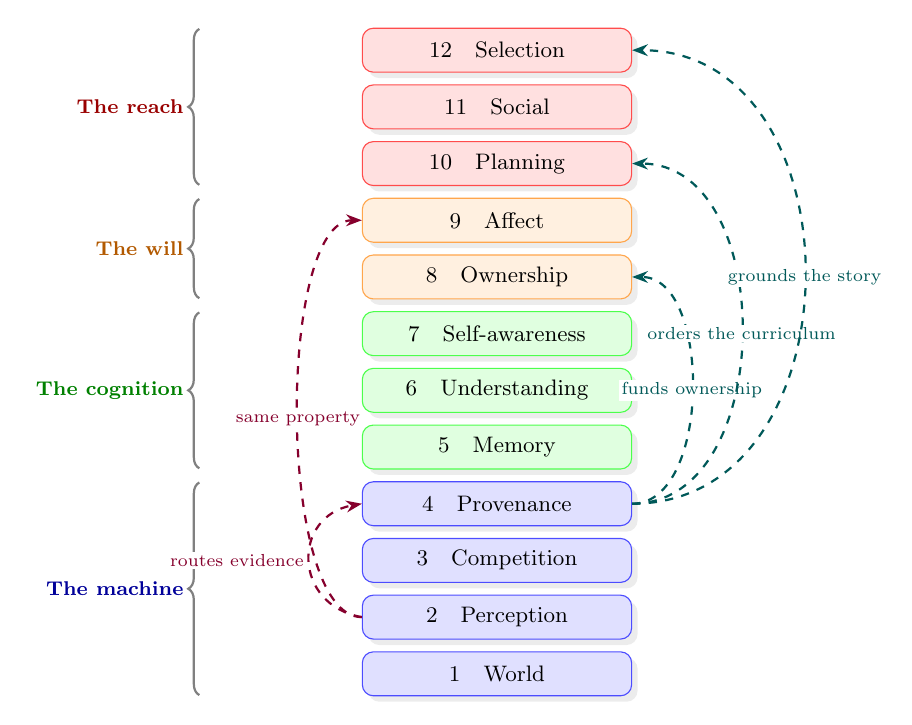
\begin{tikzpicture}[
    layer/.style={draw, rounded corners, minimum width=3.8cm, minimum height=0.62cm, align=center, font=\small, drop shadow={opacity=0.15}},
    bridge/.style={-{Stealth[length=2mm]}, thick, dashed},
    lab/.style={font=\scriptsize, fill=white, inner sep=1pt},
    scale=0.9, transform shape
]
    \foreach \i/\name/\col in {1/World/blue, 2/Perception/blue, 3/Competition/blue, 4/Provenance/blue,
                               5/Memory/green, 6/Understanding/green, 7/Self-awareness/green,
                               8/Ownership/orange, 9/Affect/orange,
                               10/Planning/red, 11/Social/red, 12/Selection/red} {
        \node[layer, fill=\col!12, draw=\col!70] (L\i) at (0, 0.8*\i) {\i\quad \name};
    }

    % Group labels, far left
    \node[anchor=east, font=\footnotesize\bfseries\color{blue!60!black}] at (-4.3, 2.0) {The machine};
    \node[anchor=east, font=\footnotesize\bfseries\color{green!50!black}] at (-4.3, 4.8) {The cognition};
    \node[anchor=east, font=\footnotesize\bfseries\color{orange!70!black}] at (-4.3, 6.8) {The will};
    \node[anchor=east, font=\footnotesize\bfseries\color{red!60!black}] at (-4.3, 8.8) {The reach};
    \draw[decorate, decoration={brace, amplitude=4pt}, thick, gray] (-4.2, 0.5) -- (-4.2, 3.5);
    \draw[decorate, decoration={brace, amplitude=4pt}, thick, gray] (-4.2, 3.7) -- (-4.2, 5.9);
    \draw[decorate, decoration={brace, amplitude=4pt}, thick, gray] (-4.2, 6.1) -- (-4.2, 7.5);
    \draw[decorate, decoration={brace, amplitude=4pt}, thick, gray] (-4.2, 7.7) -- (-4.2, 9.9);

    % Perception bridges, left
    \draw[bridge, purple!70!black] (L2.west) to[out=180, in=180, looseness=0.55]
        node[lab, pos=0.5] {same property} (L9.west);
    \draw[bridge, purple!70!black] (L2.west) to[out=170, in=190, looseness=1.6]
        node[lab, pos=0.5, left=1pt] {routes evidence} (L4.west);

    % Provenance spine, right
    \draw[bridge, teal!70!black] (L4.east) to[out=0, in=0, looseness=0.9]
        node[lab, pos=0.5] {funds ownership} (L8.east);
    \draw[bridge, teal!70!black] (L4.east) to[out=0, in=0, looseness=1.1]
        node[lab, pos=0.5] {orders the curriculum} (L10.east);
    \draw[bridge, teal!70!black] (L4.east) to[out=0, in=0, looseness=1.3]
        node[lab, pos=0.5] {grounds the story} (L12.east);
\end{tikzpicture}
\caption{The twelve layers of \gerundelle{}, in four groups. Dashed arrows are \emph{bridge
theorems}: results proved in one setting stated about another layer's own operators, ledger
or data routing. On the left, perception and affect are both instances of factorization
through a view, and Fit routes evidence to the provenance ledger by the Umwelt. On the
right, the provenance spine: the history of evidence funds ownership, orders the curriculum
for planning, and grounds every sentence of a told story.}
\label{fig:architecture}
\end{figure}

\subsection{From Implementation to Model}

The reference implementation is about 7{,}900 non-blank lines of Python in ten files. The
Lean development is about 4{,}350 lines.

Each Lean model is derived from a named Python function by a fixed recipe:

\begin{enumerate}[nosep]
    \item The mutable state the function reads (dictionaries, counters, flags) becomes an
    explicit record: a list of named fields, each with a type. Nothing is hidden.
    \item The function itself becomes a pure function of that record: same input, same
    output, every time. No side effects.
    \item Loops that collect results become set comprehensions. Dictionary lookups with
    defaults become fields. An update in place becomes a function from one record to
    another.
\end{enumerate}

\Cref{app:curiosity} shows the Python and the Lean side by side for one function (the
curiosity reading that turned out to have a bug).

A guarantee is admitted only if it is an invariant the system's own design documents or
tests already state. We do not invent promises the system does not make.

\paragraph{What this proves, and what it does not.} A theorem holds of its definitions.
The claim is that the guarantees hold of these models (the Lean functions derived from the
Python code). Whether a model faithfully captures the code is argued, not proved: the Lean
function could miss a case the Python function handles, or handle a case the Python
function doesn't. We address this as follows:

\begin{itemize}[nosep]
    \item \Cref{app:hypotheses} lists \textbf{every hypothesis} that stands in for a
    property of the code: what it assumes, and how the assumption was established (by
    reading the code or by argument).
    \item \Cref{app:coverage} lists \textbf{what each layer's model leaves out}: which
    parts of the code are not modeled, and why (too implementation-specific, or beyond the
    current development's scope).
\end{itemize}

The reader who wants to know ``did you prove the code correct?'' should read these
appendices. The answer is: we proved guarantees about models derived from the code, and we
listed every gap between the models and the code. The gaps are there to be closed, and
closing any one of them would strengthen the corresponding guarantee without changing the
others.

\begin{table}[t]
\centering
\small
\begin{tabular}{@{}lp{5.8cm}p{5.6cm}@{}}
\toprule
Layer & Lean files & Source in the reference implementation \\
\midrule
1 World & \lean{World} & \lean{civilization/potential\_world.py} \\
2 Perception & \lean{Erlangen} & design: \lean{sov\_geometry} \S1--2 \\
3 Competition & \lean{Competition} & \lean{Mind.think}, \lean{Mind.resolve} \\
4 Provenance & \lean{Ledger}, \lean{Provenance}, \lean{Firewall}, \lean{Market}, \lean{Crypto} & \sov{} spec; \lean{Territory} (\lean{Crypto}: negative result on a related secrecy conjecture) \\
5 Memory & \lean{Memory}, \lean{Quotient} & \lean{reopen}, \lean{contradict}, \lean{tell} \\
6 Understanding & \lean{Geometry}, \lean{Slot}, \lean{Operator}, \lean{Holonomy}, \lean{Confluence} & \sov{} spec \\
7 Self-awareness & \lean{Meta}, \lean{Competition} & \lean{class Meta} \\
8 Ownership & \lean{Market} & \lean{Territory.pull}, \lean{strength} \\
9 Affect & \lean{Affect} & \lean{Phases.graph} \\
10 Planning & \lean{Planning}, \lean{Pacing} & \lean{sov\_agent.py}; \lean{Mind.support} \\
11 Social & \lean{Discount}, \lean{Monad}, \lean{Integrity} & \lean{attest}, \lean{bill\_attest\_outcome} \\
12 Selection & \lean{Selection} & \lean{fiction/story.py}, \lean{rung7.py} \\
All & \lean{Bridges} & \\
\bottomrule
\end{tabular}
\caption{Lean files by layer and the Python code each model is derived from.}
\label{tab:files}
\end{table}

\subsection{How to Read the Theorems}
\label{sec:conventions}

Each layer's guarantees are presented in a fixed pattern:

\begin{enumerate}[nosep]
    \item A \textbf{Theorem} block states the guarantee in plain terms that match the Lean
    statement. The Lean name appears in \lean{typewriter} so the reader can find it in the
    development. For the flagship results, the Lean signature is given in full.
    \item A \textbf{Reading} block says what the guarantee means for the mind: what would
    go wrong if it failed, and why it matters.
    \item A \textbf{Prior work} block credits the classical result the guarantee
    instantiates: the mathematics is usually known; what is new is that it holds of this
    architecture, machine-checked.
\end{enumerate}

The formal reader can skip the Readings. The general reader can skip the Lean signatures.
Both follow the same argument.

% ============================================================
% THE MACHINE (rewrite v1)
% ============================================================

\section{The Machine: Epistemic Conservation and Invariance}
\label{sec:machine}

The first four layers answer: can the mind see, attend, and tell evidence from hearsay?
Their guarantees are about things that hold no matter what happens: conservation laws and
invariance properties that every sequence of operations preserves.

\subsection{Layer 1: World}

The world keeps one physical quantity (potential) in several places: a spring's field, a
jar's store, what each object embodies, what each object carries in motion. Every change
the world makes moves an amount from one place to another: drawing fills the jar from the
spring, spilling empties it, forming spends it to make something, launching converts it to
motion. Nothing is created or destroyed.

\begin{theorem}[Conservation of potential]
{\small\sloppy Lean: \lean{total\_runMoves}, \lean{nonneg\_runMoves}\par}
No sequence of moves changes the total potential. If every move takes at most what its
source holds, every place stays nonnegative.
\end{theorem}

\begin{reading}
The system's design document stated this as ``a theorem to prove in Lean.'' The
implementation checked it with an assertion after every tick: if the total changed, the
program crashed. Conservation held in every run reported. But ``held in every run'' is not
``cannot fail.'' The theorem is: it cannot. For any sequence of moves, in any world that
follows the rules, the total is unchanged.
\end{reading}

\subsection{Layer 2: Perception}

Two agents in the same world may perceive it differently. One distinguishes the jar's
charge level (empty, charged, brimming); another sees only empty or not-empty. The second
agent lives in a coarser world: fewer distinctions, fewer things to attend to, fewer
questions to ask. What an agent \emph{cannot distinguish} determines what it perceives.

Formally: an agent's transforms form a group $T$ acting on observations $O$. The agent's
\emph{Umwelt} (its perceived world) is the quotient $O/T$: things the agent cannot tell
apart are one point. A reading $f$ of observations is \emph{invariant} if every transform
preserves it.

\begin{theorem}[Perception is determined by invariance]
{\small\sloppy Lean: \lean{invariant\_iff\_factorsThrough},
\lean{InvariantUnder.mono}\par}
A reading of the world is something the agent can perceive exactly when it depends only on
what the agent can distinguish. More precisely: a reading is invariant under the agent's
transforms if and only if it factors through the map to the Umwelt. Enlarging the group of
transforms (making more things indistinguishable) can only remove invariants; the agent
sees less.
\begin{lstlisting}
theorem invariant_iff_factorsThrough (f : O $\to$ X) :
    Invariant T f $\leftrightarrow$ Function.FactorsThrough f
      (Quotient.mk (MulAction.orbitRel T O))
\end{lstlisting}
\end{theorem}

\begin{theorem}[Evidence routes through the Umwelt]
{\small\sloppy Lean: \lean{fit\_factors\_through\_umwelt}\par}
When the slot's feasible set is invariant under the agent's transforms, what Fit writes to
the ledger for a datum depends only on the datum's point in the Umwelt, not on which raw
observation produced it. Two observations the agent cannot tell apart produce the same
evidence.
\begin{lstlisting}
theorem fit_factors_through_umwelt
    (hF : $\forall$ (t : T) (x : R), t $\bullet$ x $\in$ F i $\leftrightarrow$ x $\in$ F i) :
    Function.FactorsThrough (fun x $\mapsto$ (Operator.fit i x c e).fiber w)
      (Quotient.mk (MulAction.orbitRel T R))
\end{lstlisting}
\end{theorem}

\begin{reading}
The first theorem says: the mind cannot perceive what its own transforms cannot tell apart.
If you can't distinguish red from green, no amount of attention will let you read a
red-green traffic light. The invariants available to you are set by the distinctions you
can make, not by the distinctions the world contains.

The second theorem connects perception to evidence. It says: two things the agent sees as
the same produce the same evidence on the ledger. The mind does not file one observation
in one slot and an indistinguishable observation in another. Evidence respects perception.

Together they mean: the agent's funded understanding is about its own Umwelt, not about
the raw world. An agent with coarse perception builds coarse understanding. An agent with
fine perception builds fine understanding. Neither is wrong; they live in different worlds.
\end{reading}

\begin{prior}
The first theorem is the factorization of invariant functions through the orbit space
\citep{LehmannRomano2005,Bronstein2021}, the principle behind equivariant networks
\citep{CohenWelling2016}. ``More transforms, fewer invariants'' is Klein's hierarchy
\citep{Klein1893}. Reading $O/T$ as an Umwelt is our interpretation of von Uexk\"ull
\citep{Uexkull2010}, following \citet{Cassirer1944}. The second theorem connects
perception to the ledger; this bridge is new.
\end{prior}

\subsection{Layer 3: Competition}

Each tick, every molecule in the working pool bids for a fixed number of slots per level.
The winners advance; the losers stay behind. Only the top level's winners are what the mind
attends to. If seven molecules bid for four slots, three of them lose, no matter how
important they are.

This is attention by construction, not by a learned allocation. The guarantees say:

\begin{itemize}[nosep]
    \item At most $k$ molecules win a level (\lean{winners\_length\_le}).
    \item A molecule that did not win has a key no higher than any winner's
    (\lean{winner\_outbids}).
    \item A molecule reaches level $L{+}1$ only by winning level $L$
    (\lean{tower\_nested}).
\end{itemize}

Not everything that shapes thought competes for a slot. A \emph{bond} (a learned link
between two kinds of thing) is in superposition each tick: it can act as an \emph{edge},
quietly connecting two molecules without taking a slot, or it can compete as a molecule in
its own right to be examined and questioned. Most of the time a recognition does its work
as an edge, below the competition. It reaches the top only when something goes wrong and
the mind needs to examine the link itself.

\begin{reading}
Competition is what makes attention scarce, and scarce attention is what makes the market
work. If every molecule could be attended to at once, there would be no tournament, no
losers, and no pressure to bid accurately. A thought that wins does so by earning its
place against everything else the mind could have attended to. The bond mechanism is why
the mind can hold learned links (``she only takes calls on sunny days'') without using a
conscious slot for each one, until one of them is questioned.
\end{reading}

\begin{prior}
The tournament borrows from Global Workspace Theory \citep{Baars1988} its limited-capacity
competition: many specialized processes compete for a stage that only a few can occupy,
with all-or-nothing access \citep{Dehaene2014}. It does not borrow the theory's broadcast,
in which the winners' contents are sent to every process, and no guarantee here concerns
one. \gerundelle{} arrives at limited-capacity competition for engineering reasons, to avoid
lock-in and to scale, and makes no claim of neural equivalence; the convergence is evidence
that the design region is good. The slot budgets (7, 5 and 4 per level) are anchored in
working-memory capacity \citep{Miller1956,Cowan2001}. The Conscious Turing Machine
formalizes global-workspace competition \citep{BlumBlum2022}; the guarantees here are the
scarcity properties of such a tournament, machine-checked.

Two terms of a molecule's bid have their own lineage. Each open site adds a constant
tension, so an incomplete thought keeps pulling until it is closed: a mechanism for the
Zeigarnik effect \citep{Zeigarnik1927}. And the bid looks forward, carrying the surprise a
molecule could still reduce, the novelty term of the free-energy principle
\citep{Friston2010}, which the design adopted to cure the tournament's lock-in. Neither is a
claim to implement active inference.
\end{prior}

\subsection{Layer 4: Provenance}

Layer~4 is the paper's spine (\cref{sec:unification}). Every other layer depends on what
this one guarantees: that evidence is trustworthy, that imagination cannot corrupt it, and
that every receipt traces back to the world.

\paragraph{The imagination firewall.}

A mind can imagine, dream, hypothesize and plan. None of it touches the funded web. The
firewall theorem says: run any interleaving of real operations, imagination-register moves
and Posit seeds. The funded web that comes out is the result of the real operations alone.
Everything imagined is invisible to it.

\begin{theorem}[The imagination firewall]
{\small\sloppy Lean: \lean{firewall}\par}
\begin{lstlisting}
theorem firewall (sops : List SysOp) (w : Web) (h : ImagWeb) :
    (SysOp.run sops (w, h)).1 =
      Operator.run (sops.filterMap SysOp.funded?) w
\end{lstlisting}
Run any interleaving of funded operators, register moves and Posit seeds: the resulting
funded web is the result of running the funded operators alone.
\end{theorem}

\paragraph{Evidence is what it says it is.}

Three guarantees about the provenance of evidence, stated separately because each
protects against a different threat:

\begin{theorem}[Imagined evidence is inert]
{\small\sloppy Lean: \lean{bid\_filter\_imagined},
\lean{run\_owner\_filter\_imagined}\par}
Removing every imagined trial from any event sequence changes no bid and no owner. A mind
that dreams, hypothesizes or speculates cannot change what it owns or what it knows by
doing so.
\end{theorem}

\begin{theorem}[Told evidence cannot be promoted]
{\small\sloppy Lean: \lean{took\_told\_le}\par}
Told-only evidence funds at most $c_0$ per trial, whatever the processing. No sequence of
operations can turn a told receipt into a lived one.
\end{theorem}

\begin{theorem}[Lived evidence comes only from the world]
{\small\sloppy Lean: \lean{replay\_mass\_le}\par}
Replaying events none of which is a lived accrual (a Fit) does not increase lived mass.
The only way to create lived evidence is to interact with the world.
\end{theorem}

\begin{theorem}[No outbound path from imagination]
{\small\sloppy Lean: \lean{no\_outbound}\par}
Every function from imagination registers to funded webs misreports lived mass on some web
with the given geometry. The asymmetry is structural: forgetting funding is always
possible; reconstructing it is impossible.
\end{theorem}

\paragraph{Self-citation and grounding.}

\begin{theorem}[Self-citation is legal but ungrounded]
{\small\sloppy Lean: \lean{wellFounded\_cites}, \lean{not\_transGen\_self},
\lean{not\_grounded\_of\_selfCited}\par}
In a log where every entry cites only earlier entries, citation is well-founded and no
entry is in its own chain. A non-root entry citing only itself or later entries is never
grounded. Circular reasoning is not prohibited; it is inert. A self-citing entry can exist; it
cannot fund anything.
\end{theorem}

\begin{reading}
Taken together, these theorems say: \textbf{provenance is conserved.} What was lived stays
lived. What was told stays told. What was imagined funds nothing. No sequence of
operations (no amount of thinking, dreaming, rehearsing or reprocessing) can upgrade the
provenance of a piece of evidence.

This is what makes the market's bids meaningful. A bid rests on evidence whose source
cannot be upgraded after the fact. And it is what makes the ownership register
trustworthy: a slot held by lived evidence was held by actual interaction with the world,
not by imagination that leaked into the ledger.

The funding gate (the precondition that a non-Fit operator must cite at least one earlier
receipt to fire) is proved necessary (\lean{not\_grounded\_of\_unfunded}): without it,
ungrounded entries appear. The gate is not a safety margin. It is a necessary condition
for grounding.
\end{reading}

\begin{prior}
The firewall is non-interference in the purge formulation of \citet{GoguenMeseguer1982}:
the imagination register is a low-integrity domain that does not interfere with the funded
web, as in type-based non-interference \citep{VolpanoIrvineSmith1996,SabelfeldMyers2003}.
Mechanized non-interference at scale has precedent in operating-system verification
\citep{Murray2013}.

Inert imagined evidence is semiring provenance with tags valued $1, c_0, 0$
\citep{GreenKarvounarakisTannen2007}. The told cap is fixed-weight discounting
\citep{Josang2016}. Lived mass is a Petri-net conservation invariant \citep{Murata1989}.
The map-back lemma is the view-complement fact \citep{BancilhonSpyratos1981,Foster2007}.

Self-citation is Kripke's ungrounded truth-teller \citep{Kripke1975}, here with
well-foundedness by construction, as in well-founded semantics
\citep{VanGelderRossSchlipf1991}. The funding gate is the well-founded support condition
of truth maintenance systems \citep{Doyle1979,deKleer1986}.

Dreaming, in the sense of sleep's replay and recombination of experience
\citep{WalkerStickgold2004} and of generative replay in machine learning \citep{Shin2017}, is
the register's natural use: replayed and recombined episodes can suggest what might fill a
slot. The firewall is what makes this safe. Nothing dreamed funds anything.
\end{prior}

% ============================================================
% THE COGNITION (rewrite v1)
% ============================================================

\section{The Cognition: Local Epistemic Geometry}
\label{sec:cognition}

The next three layers answer: can the mind remember, understand why, and notice when it is
confused? Their guarantees are mostly about local structure: what holds in the neighborhood
of one slot, one memory, one meta-observation. The exception is Understanding, whose
holonomy result characterizes when a global frame exists across all domains.

\subsection{Layer 5: Memory}

A mind that never forgets drowns in its own history. A mind that forgets everything starts
over every tick. Memory is the mechanism between: thoughts that have been fully examined
leave the active pool and are stored, and some of them come back.

A thought that closes is stored as a sealed \emph{box}, indexed by the concepts (its
\emph{keys}) that resolved it. Think of sealed envelopes with keywords written on the
outside. Time fades the ink: each key's \emph{warmth} halves every $h$ ticks it goes
unfilled, and below a threshold the key is cold and no longer checked.

A box returns to the pool in three ways:
\begin{itemize}[nosep]
    \item \textbf{Resonance.} Enough of its warm keys match what the mind is currently
    attending to. The box opens gently: the context it was closed in has partly returned.
    \item \textbf{A searching thought finds it.} A thought with an open site looks for
    what would fill it, and finds it in a stored box, behind a warm key.
    \item \textbf{Contradiction.} The world produces an outcome the box's prediction said
    would not happen. The box opens urgently, with surprise raised by how well the concept
    was understood, demanding re-examination.
\end{itemize}

Three guarantees make this precise:

\begin{theorem}[Forgetting is cooling, not deletion]
{\small\sloppy Lean: \lean{warm\_of\_le}, \lean{not\_resonates\_of\_cold}\par}
A key warm now was warm at every earlier tick. A box whose keys are all cold cannot
resonate. Memories do not vanish; they become unreachable as their context cools.
\end{theorem}

\begin{theorem}[Memory does not ruminate]
{\small\sloppy Lean: \lean{not\_reopens\_after\_resonating}\par}
A box that resonated this tick does not reopen by resonance at the next. A memory brought
back once does not immediately bring itself back again; something else must intervene.
\end{theorem}

\begin{theorem}[Lived and told memories differ]
{\small\sloppy Lean: \lean{told\_reopens\_iff}\par}
A lived box is keyed by the tags that resolved it (the concepts the mind was working with
when it closed). A moment that resembles it can bring it back by resonance. A told box
arrives already closed, with no keys of one's own, because the mind did not work it out.
No resemblance can recall it. A told box reopens if and only if the world contradicts it.
\end{theorem}

\begin{reading}
The lived/told distinction is the memory layer's version of provenance conservation. What
you worked out yourself has warming keys and can be gently recalled by a similar context.
What you were told has no keys and can only be shattered by the world saying otherwise.
``You don't own what you haven't worked out'' is not a slogan. It is a structural property
of how the box was sealed: no keys, no resonance path, only contradiction.

This is why a told belief can persist for a lifetime unchallenged; its keys never warm,
so it is never re-examined by resemblance. It reopens when the world contradicts it, or
when it is worked out: decomposed and recognised through live keys of one's own. Until
then it sits sealed, without the resonance path that would revise it gradually.
\end{reading}

\paragraph{Additional guarantees.} In the ledger's history, a lived accrual and an
eviction on the same slot do not commute (\lean{accrue\_evict\_not\_comm}): evicting after
a lived receipt writes it off, while evicting before leaves it untouched. The trace
quotient, which swaps only state-preserving events, respects ledger state
(\lean{SameTrace.replay\_eq}) and is the least congruence identifying logs of such events
that contain the same events (\lean{SameTrace.minimal}). Affective phases that fade with their question still open are
stored open and reopen when their subject returns (the design's ``Pandora'' case); this is
not yet modelled (\cref{app:coverage}).

\begin{prior}
Contradiction forcing a sealed box open is Kuhn's cycle of anomaly, crisis and revision
\citep{Kuhn1962} at the scale of a single belief: \lean{told\_reopens\_iff} says a told belief
opens only that way. That a memory does not ruminate (\lean{not\_reopens\_after\_resonating})
answers the clinical picture of rumination \citep{NolenHoeksema1991} with a mechanism: a box
that keeps resonating is held closed until it goes out of resonance.
\end{prior}

\subsection{Layer 6: Understanding}

When a mind learns something in one domain, can it carry that understanding to another?
A carpenter who understands wood grain encounters a new kind of wood. Does the understanding
transfer? Or does it distort: carry a distinction that doesn't apply, or lose one that does?

Transfer is modelled as \emph{transport}: carrying a slot's geometry from one domain to
another. Write $\tau_{ij}$ for the transport from domain $i$ to domain $j$. If you
transport from $i$ to $j$ and then from $j$ to $k$ and then from $k$ back to $i$, you
have gone around a triangle. The \emph{holonomy} of that triangle is what changed in the
round trip. If nothing changed, the triangle is \emph{flat}: the understanding transferred
perfectly. If something changed, the understanding was distorted by the path it took.

\begin{theorem}[Flat iff trivializable]
{\small\sloppy Lean: \lean{flat\_iff\_trivializable}\par}
For invertible transports given on every ordered pair of domains, every triangle has zero
holonomy (perfect transfer) if and only if there exist global coordinates (a single frame
of reference that works in every domain). Where global coordinates exist, the path doesn't
matter: going the long way around gives the same result as going directly.
\[
  \bigl(\forall i,\ \tau_{ii} = 1\bigr) \wedge \bigl(\forall i\,j\,k,\
  \mathrm{hol}(i,j,k) = 1\bigr)
  \iff
  \exists\, \varphi : \iota \to \mathrm{Perm}(G),\ \forall i\, j,\
  \tau_{ij} = \varphi_j\,\varphi_i^{-1}.
\]
\end{theorem}

\begin{theorem}[Relabel makes understanding local]
{\small\sloppy Lean: \lean{loop\_perm}, \lean{relabel\_path\_dependent},
\lean{relabel\_accumulates}, \lean{relabel\_not\_meets}\par}
Transport by meets alone (Constrain) is path-independent: it doesn't matter which order
you apply the constraints. But Relabel (translating the vocabulary from one domain to
another) makes transport path-dependent. Going around a triangle with a Relabel step can
change the understanding, and Relabel cannot be decomposed into meet steps: it is a
genuinely new operation.
\end{theorem}

\begin{reading}
Where vocabulary translation between domains is needed, there is no global frame.
Structure is inherently local, and it is the algebra's own operators that make it so (\lean{relabel\_is\_transport}, \lean{constrain\_is\_transport}).

Constrain and Exclude are confluent (\lean{p66\_constrain\_exclude}): the same constraints
applied in any order reach the same geometry. Fit does not commute with Constrain or
Archaize (\lean{fit\_constrain\_not\_perm}, \lean{fit\_archaize\_order}): the order of
evidence and narrowing matters for the ledger, even when it doesn't matter for the
geometry.

A discovery has an epistemic order; the steps cannot be rearranged and produce the same
result. The holonomy theorem proves this for the algebra's own operators: transport by
Relabel is path-dependent, and that path-dependence is not removable. Going around the
triangle the long way is not the same as going directly, because Relabel is not a meet
step.
\end{reading}

\begin{prior}
The flat-iff-trivializable theorem, on the complete graph of domains, is the coboundary
criterion for a non-abelian 1-cocycle \citep{Giraud1971}, the discrete analogue of a pure
gauge in lattice gauge theory \citep{Wilson1974}, known in vision as cycle consistency or
synchronization \citep{Singer2011,PachauriKondorSingh2013,HuangGuibas2013,GaoBrodzkiMukherjee2021}. Local consistency without a
global section is the subject of sheaf methods
\citep{HansenGhrist2019,AbramskyBrandenburger2011}. Relabel's underivability from meets
is an instance of \citet{Howie1966}: products of idempotent transformations are never
non-identity permutations.
\end{prior}

\subsection{Layer 7: Self-awareness}

A mind that cannot notice its own confusion stays confused. A mind that monitors its own
processing at the cost of the processing itself notices everything and does nothing.
Self-awareness is the layer that negotiates between these.

The mind forms \emph{meta molecules}: molecules about another molecule's state. ``I am
stuck,'' ``I am looping,'' ``this thought gives two different outcomes and I don't know
why.'' Meta molecules compete; they do so only among themselves, in their own dedicated slots,
so they never crowd out regular thoughts.

Two hazards govern this layer, each a design rule guarding against a failure mode the
design documents name:

\paragraph{The mirror trap.} A meta molecule that refreshes itself by re-detecting the
state it was about would consume a slot, contribute nothing, and resist removal because the
state it reported was still true: rent without yield, a mirror that reflects without
acting. The design guards against this: every meta molecule carries a \emph{prediction}
about its subject, with a \emph{deadline}. It lives by being right about the future, not
by re-observing the present. A prediction confirmed extends the deadline. A prediction
refuted kills the molecule. No re-detection extends its life.

\begin{theorem}[The mirror trap is closed]
{\small\sloppy Lean: \lean{detect\_standing},
\lean{deadline\_changes\_only\_by\_confirmation}, \lean{refuted\_dropped},
\lean{check\_before\_deadline}\par}
Detecting a standing state again does not extend a meta molecule's life. The deadline moves
only when the prediction is confirmed. A refuted molecule is dropped. None outlives its
deadline undecided.
\end{theorem}

\paragraph{One-way aboutness.} A meta molecule about a thought should not inflate the
thought it is about. Without a guard, ``I notice this'' could boost the thing noticed,
creating a feedback loop: noticing makes the thought louder, which makes the noticing more
relevant, which makes the thought louder. The design rules this out.

\begin{theorem}[Meta cannot inflate base]
{\small\sloppy Lean: \lean{base\_filter\_meta}, \lean{partner\_not\_meta},
\lean{bid\_ignores\_meta}\par}
Meta molecules compete in separate slots and never displace a thought. A thought never
binds to a meta molecule. Adding meta molecules never changes a thought's bid. Meta
operations such as parking or splitting do act on their subject, but the bid (the
measure of competitive strength) is unaffected.
\end{theorem}

\begin{reading}
Self-awareness is not free. The meta molecule must \emph{win} a slot to act; it must
outcompete other meta molecules, not regular thoughts. The capacity to notice confusion
exists whether or not confusion is noticed: the meta molecule is in the pool, but it might
lose to a more urgent meta-observation. This is why you can be stuck without knowing you
are stuck, and why the realization ``I'm going in circles'' surfaces only when the meta
molecule finally wins.

The aboutness guarantee protects against the architectural version of rumination: a mind
that notices its own anxiety and is made more anxious by noticing. The one-way rule keeps
the observation channel silent: the camera doesn't disturb the wildlife.
\end{reading}

\paragraph{Additional guarantees.} A meta molecule binds only to its subject
(\lean{meta\_partner\_is\_subject}), and the tower of meta levels is bounded in depth
(\lean{emitDepth\_le}). Operations such as parking or splitting fire only for a meta
molecule among the top winners (\lean{operated\_mem\_top}), and kinds with an operation
take those slots first (\lean{operable\_win\_first}). A want is never parked
(\lean{not\_goal\_of\_parkable}). When a thought's outcomes go two ways, splitting it on a
boundary partitions its outcomes; mending a wrong split restores them, keeping any outcomes
gathered since (\lean{mem\_split\_iff}, \lean{unify\_differentiate},
\lean{unify\_keeps\_later}).

\begin{prior}
Splitting a conflated thought is Piaget's accommodation \citep{Piaget1952}: a schema revised
because the world will not fit it. The conflations it acts on are the bimodal outcomes Carey
documents in children's conceptual change \citep{Carey1985}, and mending a wrong split is
the revision run the other way. A meta layer that notices and operates on the system's own
representations is representational redescription in the sense of
\citet{KarmiloffSmith1992}.
\end{prior}

% ============================================================
% THE WILL (rewrite v1)
% ============================================================

\section{The Will: Non-commutative Territorial Dynamics}
\label{sec:will}

The previous layers explain how a mind perceives, attends, remembers and understands. None
of them explains why the mind acts at all. Curiosity ranks questions without originating
wants. Understanding fills slots without saying which slots matter. Something else is needed:
a reason to push.

The answer is territory. An agent acts to hold what it perceives as its own.

\subsection{Layer 8: Ownership}

Territory is whatever the agent perceives as its own: a body, a place, an object, an idea, a
relation, or a slot in another mind. Being on someone's mind, living rent free in their
thoughts, is territory too: a relation in their understanding whose filler is the agent.
The reference implementation models it as a slot another mind holds open for the agent
(until she answers, the agent is not on her mind), and credits actions to it; the Lean
development does not yet cover it, and the theorems below concern regions of the world.

For each region of the world, the territory register tracks how the agent perceives its
holding, and opens an ownership slot where the boundary is incomplete. Three slot kinds
govern how hard each region pulls on the mind's attention:

\begin{itemize}[nosep]
    \item \textbf{Unclaimed} (never tried): ``What happens if I push here?'' A spring the
    agent has never drawn from, an object it has never touched. It pulls at
    $\mathrm{curiosity}\cdot\kappa/(\kappa + \mathrm{other})$; less when something else
    already moves the region, because a region that moves on its own is harder to claim.

    \item \textbf{Control} (tried, not yet taking, or wanted): ``What blocks it?'' A lid
    the agent has pushed and that didn't move, a want that hasn't been met. It pulls harder
    the longer the agent has pursued it: $1 + \mathrm{tried}/(\mathrm{tried} + \kappa)$.

    \item \textbf{Lost} (held once, fallen back): ``What took it?'' A toy the agent played
    with and that was carried away. It pulls hardest of all: $1 + \mathrm{held}$. The more
    was held, the more there is to lose. This is loss aversion as a structural property,
    not as a bias parameter.
\end{itemize}

A held region that something else also moves, or on which a claim has just failed, opens a
\emph{contested} slot. The affect layer reads it.

Two guarantees define the ownership layer's dynamics:

\begin{theorem}[Funding is order-free; ownership is not]
{\small\sloppy Lean: \lean{bid\_perm}, \lean{ownership\_order\_dependent}\par}
A bid depends only on the multiset of trials; the order of the evidence doesn't matter
for what the agent knows. But ownership depends on the sequence: the same three events
(a lived take, a close, a contradiction) in two different orders leave a slot open in one
case and held in the other.
\end{theorem}

\begin{reading}
This pins down exactly where the architecture's non-commutativity lives. What you know is
the same regardless of the order you learned it in: bids are order-free. But who holds
what depends on history: a slot taken and then contradicted ends open, while the same slot
contradicted and then taken ends held. Evidence commutes. Territory doesn't. History
matters for ownership the way it matters for a treaty: the last event, not the first,
determines what holds.
\end{reading}

\begin{theorem}[The pull order, and its temperament inversion]
{\small\sloppy Lean: \lean{pull\_order}, \lean{restless\_inverts}\par}
With curiosity at most 1, given that the lost slot has held at least once and the control
slot has been tried: lost pulls harder than control, control harder than unclaimed. With
curiosity at 2, an unclaimed region that nothing else moves outpulls every control slot.
\end{theorem}

\begin{reading}
The pull order IS temperament, with proved boundaries. In the default range (curiosity at most 1), lost slots pull harder than control slots,
which pull harder than unclaimed ones: the mind attends to what it lost, then to what it
is pursuing, then to what it hasn't tried. In the restless range (curiosity at 2), an
unclaimed region that nothing else moves pulls harder than any control slot. The order is proved for curiosity at most 1, and its
inversion at curiosity 2; the gap between is open. Different parameter settings produce
different characters with proved structure, not accidental variation.
\end{reading}

\begin{prior}
The split between commutative aggregation and order-dependent revision is standard in
belief revision \citep{AlchourronGardenforsMakinson1985,DarwichePearl1997}. In reinforcement
learning, exploration is a bonus added to reward: a count-based novelty term
\citep{StrehlLittman2008,Bellemare2016} or an intrinsic-reward weight
\citep{Pathak2017,OudeyerKaplanHafner2007}. Here it is not a bonus. An unclaimed region is
an ownership slot competing for attention like any other, and how strongly it pulls is a
matter of temperament. What it shares with artificial curiosity
\citep{Schmidhuber1991,OudeyerKaplanHafner2007} is the intuition that curiosity is about what
could be learned, not a hand-coded reward.

That loss pulls hardest follows the revised ethology of the wolf pack: the ``alpha'' is not a
dominant animal but the one with the most to lose \citep{Mech1999}. Territory is about what
is held, not about dominance. Ownership as the foundational motivation meets
self-determination theory's three needs \citep{DeciRyan1985,RyanDeci2000}: autonomy is
control (the agent's push works), and competence is understanding funded by control slots.

The market is an auction for control in the
lineage of \citet{Baum1999} and \citet{Wellman1993}; funding here is provenance-weighted
evidence, not transferred money.
\end{prior}

\subsection{Layer 9: Affect}
\label{sec:affect}

Emotions are not labels applied after the fact. They are states of the ownership register,
read off its graph each tick. The agent does not decide to feel frustrated. The register
says: a live slot has failed twice running. That IS frustration.

Each tick, the phases are read from a \emph{snapshot}: the register's open and live slots,
each region's history of failures, the claims that took, and a context of what lies outside
the register (who won the competition, whom understanding blames).

\begin{theorem}[The phases]
{\small\sloppy Lean: \lean{mem\_graph\_frustration},
\lean{anxiety\_of\_one\_failure}, \lean{mem\_graph\_joy},
\lean{live\_empty\_of\_calm}, \lean{mem\_graph\_curiosity}\par}
Each emotional phase has an exact formation condition:
\begin{itemize}[nosep]
    \item \textbf{Frustration:} a live slot (control or contested by its own failure) with
    two or more failures running. The claim keeps failing.
    \item \textbf{Anxiety:} one failure on a contested slot. A held region under pressure.
    \item \textbf{Joy:} an instance closed because a claim took. The push worked.
    \item \textbf{Calm:} nothing is live. No open slot, no unfinished business.
    \item \textbf{Curiosity:} an unclaimed live slot won the ownership track. Something
    untried pulled hard enough to win attention.
\end{itemize}
\end{theorem}

\begin{theorem}[Which layer each phase reads]
{\small\sloppy Lean: \lean{register\_phases\_factor},
\lean{curiosity\_not\_factor}, \lean{curiosity\_factors},
\lean{anger\_not\_factor}\par}
\begin{lstlisting}
def view (s : Snapshot) : Register $\times$ Memory := (s.reg, s.mem)
theorem register_phases_factor :
    FactorsThrough (reading registerKinds) view
theorem curiosity_not_factor :
    $\neg$ FactorsThrough (reading {.curiosity}) view
theorem curiosity_factors :
    FactorsThrough (reading {.curiosity}) (fun s $\mapsto$ (s.reg.live, s.ctx.top))
theorem anger_not_factor :
    $\neg$ FactorsThrough (reading {.anger}) view
\end{lstlisting}

Frustration, anxiety, sadness, joy, calm, gratitude and resignation all factor through
the register and the previous tick: they depend only on what the agent holds, not on what
it thinks or whom it blames.

Curiosity does not factor through the register alone. It also reads the competition's
winners: curiosity depends on what won attention, not just on what is unclaimed.

Anger does not factor through the register alone either. It also reads understanding and
the meta layer: anger is anger \emph{at someone}, and whom to blame is inferred from who
was seen taking what was lost and, through understanding, from whatever keeps the state a
failing claim depends on.
\end{theorem}

\begin{reading}
The positive result and the two negative results together form a \textbf{map of how
affect connects to the other layers}. Most emotions live in the ownership register alone.
Curiosity reaches into competition. Anger reaches into understanding. The map is proved,
and it is sharper than the theorem we first set out to prove.

Co-occurrence is not causation: getting the right emotion in the right place is not the
same as knowing why it is there. The proved map is the difference. It does not just
correlate phases with states; it identifies the exact conditions and the exact layers each
phase reads, and it proves which phases break the factorization property and why.

The guarantee we first proposed was: two minds alike in ownership feel alike. It was false,
as the code showed: curiosity reads the competition's winners, anger reads understanding.
The true statement is the map above: which phases read which layers. This is the second
lesson of the cautionary tale (\cref{sec:intro}).

The mathematical structure is the same one that governs perception (Layer~2).
\lean{FactorsThrough} is the same property that, with the Umwelt's quotient map in place
of \lean{view}, says ``a reading is something the agent can perceive exactly when it is
invariant.'' Applied here, it says: ``a phase is something the ownership register
determines exactly when it factors through the register.'' Perception factors through the
Umwelt; affect factors through the ownership register. Same property, two levels. Bridge
theorem: \cref{sec:unification}.

Anger is the instructive case for why the map matters. Blame can spread: each new thing
that fills a blocked goal's ``caused by'' slot gets a copy of the anger, and those copies
compete in the thoughts' own slots (the cascade the design calls a \emph{cancer of the
mind}). A grounded copy (one whose blame the records support) closes when its goal is met.
A copy whose blame the records do not support escapes that closure and only fades.
\lean{anger\_not\_factor} is the formal trace of this: anger cannot be read off ownership
alone because blame is not an ownership fact.
\end{reading}

\begin{prior}
Phases are appraisals made executable \citep{Lazarus1991,Scherer2001}: each is a structured
evaluation whose anchor is what is appraised and whose kind is the result. In the sense of
\citet{Damasio1994}, they are not noise on reasoning but what lets the agent prioritize: they
redirect which questions it pursues. The spread of ungrounded anger copies through the
thoughts' slots is rumination \citep{NolenHoeksema1991} given a mechanism.
\end{prior}

% ============================================================
% THE REACH + UNIFICATION (rewrite v1)
% ============================================================

\section{The Reach: Geodesic Agency}
\label{sec:reach}

The last three layers answer: can the mind plan far ahead, learn from others, and tell
what happened? Their guarantees are about paths: valid paths through a space of
understanding, valid paths from one mind to another, and valid paths through a story.

\subsection{Layer 10: Planning}

\paragraph{Sub-wants: when the goal is too far.}

The planner looks three steps ahead. A mind on the moon that wants to go home faces a
seven-step chain: unmake the husk, draw from the pool, draw again, form the lantern, fuse
it onto the skiff, fill the flask, launch. Seven steps. Three-step horizon. The goal is
invisible from where the mind stands.

The solution: the mind sets a nearer goal (a \emph{sub-want}) and keeps the distant want
on a stack. ``I need the pool glimmering before I can light the skiff, so I'll want that
first.'' Each sub-want is within the planner's horizon. The mind reaches it, pops the
stack, and the next sub-want takes over.

\begin{theorem}[Sub-wants are bounded]
{\small\sloppy Lean: \lean{inv\_run}, \lean{drops\_le\_card}\par}
Along any run, the sub-want stack is at most four deep. No want appears on the stack
twice. No sub-want once dropped is set again. Over finitely many facts, a run drops at
most as many sub-wants as there are facts.
\end{theorem}

\begin{reading}
The stack is bounded and non-repeating: no want appears twice on the stack, and a dropped
sub-want is never set again. A mind chasing a far goal cannot loop on the same sub-want
or accumulate an unbounded stack; each step either advances or exhausts a distinct option.
\end{reading}

\paragraph{Constraint convergence: finding the one that survives.}

The mind does not search for solutions. It searches for \emph{constraints}; the
solution is the one left standing when the constraints converge.

A hand reaching for a hot mug full of coffee: the body is hot (learned from a burn), the
rim is chipped (learned from a cut), it must not tilt (learned from a spill), the bottle
blocks one side (learned from a knock). Under those constraints, perhaps one grasp survives:
the handle, from the right, fingers through.

\begin{theorem}[JustOne]
{\small\sloppy Lean: \lean{justOne}\par}
When exactly one attempt meets every live constraint and each other attempt misses at
least one, that attempt is the unique best supported.
\end{theorem}

\begin{reading}
The solution is not computed. It is \emph{noticed}: the one attempt that meets every
constraint wins the tournament by simultaneous support. The mind never searched the space
of grasps. It searched the space of constraints, which is small, and the grasp was what
was left.

Failures are constraint revelations, not negative signals. A failure that reveals a new
constraint is worth more than a success that confirms what was already known: the success
changes nothing about which attempt survives, while the failure shrinks the space the next
attempt must occupy.
\end{reading}

\paragraph{The curriculum is a geodesic.}

What can be learned in what order is a structured space. Each concept has prerequisites,
and a valid curriculum visits them in order.

\begin{theorem}[Every valid curriculum is a shortest path]
{\small\sloppy Lean: \lean{card\_learn}, \lean{never\_enters},
\lean{reachable\_of\_downClosed}\par}
A valid curriculum adds one concept per step, never enters a prerequisite cycle, and
reaches every achievable state when prerequisites form a strict order. No valid path
wastes a step.
\end{theorem}

\begin{reading}
The mind's understanding grows along the shortest path that respects its prerequisites.
A prerequisite cycle is unreachable (proved, not assumed). The curriculum can't get stuck
in a loop and can't take a detour. Every achievable state of understanding can be reached
by some valid curriculum.

The cost of search scales with ignorance, not with the search space. The more the mind
understands (the more slots are funded, the more constraints are live), the fewer
candidates survive to be tested. Understanding is what makes search unnecessary. That is
what understanding is for.
\end{reading}

\begin{prior}
Valid curricula are the learning words of the ordinal knowledge space of the prerequisite
relation \citep{DoignonFalmagne1985,FalmagneDoignon2011,CosynUzun2009}, the case with
conjunctive prerequisites only. A concept on the fringe (unknown, with every prerequisite
known) is what the learner is ready for next: Vygotsky's zone of proximal development
\citep{Vygotsky1978}, made exact for this case.
\end{prior}

\subsection{Layer 11: Social}

Minds exchange knowledge by Pose (sending a geometry to another mind) and Attest
(importing another mind's receipts at a discount). The central question: when knowledge
passes from one mind to another, what happens to its provenance?

\begin{theorem}[Testimony stays testimony]
{\small\sloppy Lean: \lean{lamarckian\_ill\_graded}\par}
The arrow pairing Pose's geometry move with a lived accrual does not have Pose's grade:
it is ill-typed in the graded monad. Knowledge passed between minds arrives as told, never
as lived.
\end{theorem}

\begin{reading}
A parent who has learned by doing cannot pass that doing's provenance to a child. The child
receives the content (what the parent learned) but not the experiential warrant. The
child's receipt is told, at half weight, and must be tested to become the child's own.

Pose's grade is empty because of what Pose is: it shares structure, not experience. With
that grade, no arrow that writes a lived event can carry it, so the Lamarckian pairing
(inheriting the experiential warrant of acquired characteristics) is a type error in the
graded monad, not a rule that could be relaxed without changing what Pose is. The provenance firewall extends across lifetimes, not just across the
imagination boundary.

Tacit knowledge is only tacit when it lives in weights. When it lives in funded constraints
with provenance, it is inspectable: the expertise and its justification are the same
structure. A bond that fires below the competition's top level still carries the trials
that funded it. Every constraint the mind acts on has a receipt.
\end{reading}

\paragraph{Additional guarantees.} The two-stage attestation discount stays in $[0,1]$ at
every stage of calibration (\lean{discount\_mem}), so the evidence guarantees of Layer~4
apply to testimony. Against an adversary that controls a signed log, an honest agent's
viewed lived mass is at most what it signed (\lean{honest\_livedMass\_le}); the adversary
can only truncate (\lean{accepted\_take}).

\begin{prior}
The grading is a graded monad in the sense of \citet{Katsumata2014}, presented as an
effect predicate on a state-writer monad
\citep{LucassenGifford1988,FujiiKatsumataMellies2016,OrchardPetricek2014}. The Lamarckian
distinction is from cultural evolution theory \citep{BoydRicherson1985}; what is not
transmitted is the experiential warrant \citep{Kronfeldner2007}.
\end{prior}

\subsection{Layer 12: Selection}

A mind that acts in a world produces a history of beats: what it did, what happened, what
it realized, what it felt. The story layer selects which beats to tell, in what order, and
the fiction pipeline prints each one as a sentence with an intended structural skeleton.
The determination system reads each sentence back: a sentence passes only if a reading
has the shape the construction intended.

\begin{theorem}[A story is a provenance log]
{\small\sloppy Lean: \lean{sourced\_append}, \lean{sourced\_rebuild},
\lean{scene\_wellFounded}, \lean{scene\_not\_transGen\_self}\par}
Each told sentence cites only earlier sentences. Every rebuilding pass preserves this.
Dependence among sentences is well-founded, and no sentence depends on itself.
\end{theorem}

\begin{theorem}[A deus ex machina scores zero]
{\small\sloppy Lean: \lean{value\_eq\_zero\_of\_unforeshadowed},
\lean{value\_pos\_iff}\par}
The author's score is suspense held late times the rise of the ending's probability. An
ending no likelier just before it became certain than at the start earns nothing: it came
from nowhere. Value is positive exactly when there is both suspense (the reader didn't
know) and foreshadowing (the text moved the reader toward it).
\end{theorem}

\begin{reading}
A story is the same kind of structure as evidence. Each sentence cites what came before
it, and nothing cites the future. The ledger's well-foundedness theorem, proved once for
evidence in Layer~4, is the same theorem that grounds a told story in Layer~12.

The deus ex machina theorem says: value requires both uncertainty and convergence: the
same tension between suspense and foreshadowing that every storytelling manual prescribes,
here proved as a product whose factors are both necessary.

Ownership is load-bearing for narrative arc: the tension in a told story comes from
failing claims, and resolution comes from claims that took. The selection layer does not
impose narrative shape on the history; the ownership register already has it. The author
reads it off.
\end{reading}

% ============================================================
% ANALYSIS: THE UNIFICATION (rewrite v1)
% ============================================================

\section{Analysis: The Unification}
\label{sec:unification}

The guarantees above were proved layer by layer. Several were first stated over generic
structures: groups acting on sets, permutations between domains, trials with weights,
prerequisites with an ordering. Bridge theorems then stated each result about the
architecture's own operators, ledger and data routing. The result: six areas of
mathematics that rarely cite one another in the literature describe the same system.

\subsection{Bridge Theorems}

A bridge theorem takes a result proved generically and states it about the architecture's
own operators, ledger and data routing. \Cref{tab:bridges} lists them.

\begin{table}[t]
\centering
\small
\begin{tabular}{@{}p{2.8cm}p{9.5cm}p{3.2cm}@{}}
\toprule
Layers joined & What the bridge says & Lean \\
\midrule
Understanding & Relabel and Constrain are the transport steps of the holonomy theory:
the locality results are about the algebra's own operators, not abstract permutations. &
\lean{relabel\_is\_transport}, \lean{constrain\_is\_transport} \\[4pt]
Provenance $\to$ Ownership & A slot's market funding is its lived accruals at weight 1
plus its attested imports at $c_0$; imagined content yields no trial. The provenance
layer's evidence is the ownership layer's currency. &
\lean{took\_trials} \\[4pt]
Provenance $\to$ Planning & Reading the ledger in order is a valid curriculum. Every
valid curriculum over it is a geodesic. The history of evidence is the mind's own
textbook, in the right order. &
\lean{reading\_in\_order\_valid}, \lean{ledger\_curriculum\_geodesic} \\[4pt]
Provenance $\to$ Selection & A story is a provenance log: the well-foundedness theorem
for evidence is the same theorem that grounds sentences. &
\lean{scene\_wellFounded} \\[4pt]
Perception $\to$ Provenance & When a slot's feasible set is invariant under the agent's
transforms, Fit routes evidence by the Umwelt: two observations the agent can't distinguish
produce the same filing. &
\lean{fit\_factors\_through\_umwelt} \\[4pt]
Perception $\to$ Affect & Perception factors through the Umwelt; the register phases
factor through the ownership register. Same property, two levels. &
\lean{invariant\_iff\_factorsThrough}, \lean{affect\_factorsThrough} \\
\bottomrule
\end{tabular}
\caption{Bridge theorems. Each joins two layers by stating a stand-alone mathematical result
about the architecture's own operators, ledger or data routing. Four of the six pass through
Provenance (Layer~4): the ledger is the spine.}
\label{tab:bridges}
\end{table}

\subsection{Perception and Affect Are One Property}

The last row of the table is the clearest instance of the paper's thesis. Perception and
affect share one mathematical structure: factorization through a view.

For perception: a reading of the world is something the agent can perceive exactly when it
depends only on what the agent can distinguish. The view is the Umwelt.

For affect: an emotional phase is something the ownership register determines exactly when
it depends only on what the register holds. The view is the register.

Neither result is derived from the other. What is proved is that both are instances of one
universal property. And the negative results (curiosity doesn't factor, anger doesn't
factor) tell you exactly where the property breaks and which other layer each failing
phase reaches into.

Perception factors through the Umwelt; the register phases factor through the ownership
register. Same structure. Two levels.

\subsection{Provenance as the Spine}

Four of the six bridges pass through Layer~4. The ledger's well-foundedness, proved once
for evidence, is the same theorem that grounds a told story. The ledger read in order is a
curriculum. The ledger read per slot is the market's funding. And Fit, the only source of
lived mass, writes to the ledger by the Umwelt.

Provenance is not one layer among twelve. It is the structure the others are stated in. The
history of what happened, and what it was worth, is the backbone from which ownership draws
its funding, planning draws its curriculum, and selection draws its ground. Remove the
provenance layer and four of the six bridges lose their footing.

The stand-alone modules (\lean{Erlangen}, \lean{Holonomy}, \lean{Pacing}, \lean{Market})
were initially disconnected from the \sov{} web. Bridge theorems were then written to state
each result about the architecture's own operators and ledger. The unification is what
those bridges revealed: provenance is the spine.


% ============================================================
% RELATED WORK, DISCUSSION, CONCLUSION (rewrite v1)
% ============================================================

\section{Related Work}
\label{sec:related}

\paragraph{Broad architectures of mind.}

Several architectures describe a mind across many faculties: ACT-R
\citep{Anderson2004}, LIDA \citep{Franklin2014}, CLARION \citep{Sun2016}, NARS
\citep{Wang2013} and Sigma \citep{RosenbloomDemskiUstun2016}, with the Standard Model of
the Mind as a consensus synthesis \citep{LairdLebiereRosenbloom2017}; see
\citet{LangleyLairdRogers2009} and \citet{KotserubaTsotsos2020} for surveys. Their breadth
is architectural: many components in one system. Sigma's ``grand unification'' is one shared
computational substrate, not shared theorems. None of these is mechanized in a proof
assistant, and none connects its faculties by proved bridges.

Single-principle theories unify by reduction: the free-energy principle accounts for
perception, action and attention with one variational quantity \citep{Friston2010}, recast
categorically by \citet{Smithe2022}; the Conscious Turing Machine formalizes
global-workspace attention as a competition for broadcast \citep{BlumBlum2022}; universal
intelligence is fully formal but describes no faculties \citep{LeggHutter2007}.

\gerundelle{} unifies differently: not one substrate and not one principle, but named
structures proved to hold across layers, connected by bridge theorems, and every result
machine-checked.

\paragraph{Machine-checked agents.}

Agent verification is mature but targets programs, not minds. BDI agent programs are
model-checked \citep{Bordini2006,Dennis2012,Dennis2018}, including the decision layer of
autonomous systems \citep{Dennis2016}; \citet{Luckcuck2019} survey the field. In a proof
assistant, \citet{Jensen2021,Jensen2022} formalizes the GOAL agent language in Isabelle/HOL.
\citet{McCann2026} mechanizes in Coq the governance safety of AI workflow systems.
Mechanizations of single components cover Markov decision processes
\citep{Vajjha2021,SchaefflerAbdulaziz2023}, AGM belief revision \citep{Fouillard2021},
and non-interference for hardware \citep{AzevedodeAmorim2016}.

None of these spans perception through narrative. Verifying an agent language proves that
programs in that language behave correctly. Verifying an architecture of mind proves that
the architecture's own layers compose correctly: that imagination cannot corrupt evidence,
that perception determines what evidence is filed, that a told story is grounded in the
history it tells. The levels of analysis are different.

\paragraph{Emotion and ownership.}

Logical formalizations of appraisal theory define emotions over belief, desire and ideals
\citep{AdamHerzigLongin2009,SteunebrinkDastaniMeyer2012}; EMA computes appraisal from
plan structure \citep{GratchMarsella2004}; and \citet{Reisenzein2013} argues for formal
specification of emotion theories. Closest to reading affect off holdings, EBDI defines
fear and anxiety over resources at risk \citep{PereiraOliveiraMoreira2008}. Active
inference ties valence to the rate of change of the quantity perception minimizes
\citep{JoffilyCoricelli2013}. Mechanical checking of emotion models has so far been
finite: answer-set verification of appraisal trajectories \citep{BrannstromNieves2025} and
trace checking of a formalized model of Damasio \citep{BosseJonkerTreur2008}.

\gerundelle{}'s contribution here is twofold. First, reading affect off the territory
register rather than off beliefs and desires: the emotional phases are states of what the
agent holds, not of what it thinks. Second, a proved map of which layer each phase reads:
including the negative results (curiosity and anger do not factor through the register),
which tell you exactly where the nice property breaks. We know of no prior
proof-assistant mechanization of an affect model.

\paragraph{Narrative.}

Story generation by planning links events by causal structure
\citep{RiedlYoung2010,WareYoung2014}; emergent narrative lets stories arise from
simulated agents \citep{EvansShort2014}. Suspense has been modelled by escape plans
\citep{ONeillRiedl2014}, by foreshadowing \citep{BaeYoung2008}, and as variance in an
audience's beliefs \citep{ElyFrankelKamenica2015}. Narrative has been verified before:
\citet{Bosser2011} use Coq to prove properties of every plot variant of a story encoded
in linear logic, and plot spaces have been model-checked
\citep{ThompsonBattlePadget2015}.

These verify a plot space a designer authored. \gerundelle{} proves well-foundedness of
telling for every history of a simulated mind, and characterizes when a told story has
value: suspense times foreshadowing, with a proved theorem that an unforeshadowed ending
scores zero.

\medskip
The prior work behind each individual result is credited in the \emph{Prior work}
paragraphs of \cref{sec:machine,sec:cognition,sec:will,sec:reach}.

% ============================================================
\section{Discussion}
\label{sec:discussion}
% ============================================================

\paragraph{Why does unification matter?}

A guarantee proved about one layer in isolation says nothing about how the layers compose.
The bridges are where composition is checked.

The firewall would be vacuous if the market's funding did not come from the ledger: what
good is an imagination boundary if ownership draws on a different source? The story's
well-foundedness would be a separate fact if sentences were not provenance entries: what
grounds the story is the same structure that grounds evidence.

Stating the classical results on one architecture turns them from analogies into
constraints on a single design. Non-interference in the literature is a property of
security monitors. Here it is a property of imagination. Learning spaces in the literature
describe what a student can learn next. Here they describe what a mind's own history
teaches it. The mathematics is the same. The application is new, and the connections between
applications are proved.

A system that explains things it was not designed to explain is a sign the abstraction is
real. Each piece of \gerundelle{} was built for its own reasons: the story layer to tell
what a mind did, the affect layer to read its territory, the ledger to keep its evidence
honest. The bridges were written to connect them, and what they found was not built in: a
told story's grounding is the ledger's own theorem, and affect has the same structure as
perception. Pieces built for their own reasons chained into something none of them was
designed for.

\paragraph{What the architecture fixes.}

\Cref{tab:paradigms} contrasts \gerundelle{} with symbolic and statistical AI by what each
fixes in advance and what each leaves to experience.

\begin{table}[t]
\centering
\small
\begin{tabular}{@{}p{2.6cm}p{3.9cm}p{3.9cm}p{4.2cm}@{}}
\toprule
 & Symbolic AI & Statistical AI & \gerundelle{} \\
\midrule
What is fixed & What is known: rules, axioms, ontologies & Architectural biases
(attention, convolution); content is learned & The mechanics of knowing: operators,
competition, provenance, territory \\[3pt]
What is not known & A missing rule or a failed query: a gap with no shape & Diffuse
probability over outcomes & A structural open slot: defined by its type and its
relations to what is known, which narrow its feasible set; it pulls on attention \\[3pt]
How it learns & Deduction, and knowledge written by hand & Global optimization over large
corpora & Local funding: acting in a world and filing receipts \\[3pt]
When the world contradicts it & Every conclusion resting on the changed premise is
retracted and rebuilt (managed by truth maintenance \citep{Doyle1979}) & Further training;
invariants and facts move together & The contradicted slot or box reopens (that revision
stays confined to it is a design property, \cref{sec:discussion}) \\[3pt]
Its own invariants (imagining is not seeing; hearsay is not experience) & Written as rules,
if at all & Learned, and held statistically & Proved for every sequence
(\lean{firewall}, \lean{took\_told\_le}) \\
\bottomrule
\end{tabular}
\caption{What each approach fixes in advance and what it leaves to experience.}
\label{tab:paradigms}
\end{table}

\paragraph{The architecture in use.}

Fiction, code, embodiment and civilization run on the same architecture, because the same
operations apply in each: push, observe the outcome, fund a slot, discover a condition,
transfer by shape. The mind and the algebra stay fixed; only the world changes. The
domains are projections, not separate systems. Five tracks run on the reference
implementation; their results are empirical, measured in runs, not proved.
\begin{itemize}[nosep]
    \item \textbf{Civilization.} Populations of minds live in worlds whose physics is a
    parameter, and the civilization is whatever they produce there. A what-if question
    (what if there were no sunlight?) is a pair of runs that differ only in physics, and
    whatever institution, conflict or technology appears can be traced through provenance
    to the constraint that produced it. Fifteen rungs (P0 to P14) have been run, through
    populations, sub-wants, locks, grievance and retaliation.
    \item \textbf{Fiction.} A mind's encounter with a world, told by an author: fiction
    generated from first principles (a world, a mind, a ledger and author rules), with every
    sentence traceable to the world state that caused it, and no copyrighted text. The
    ladder's first eight rungs run from one character with one want to several endings held
    open; on every rung the reference configuration's told story reads back at 1.00, and
    the pipeline produces corpora.
    \item \textbf{Code.} The code is a mind, not something a mind writes: a program's
    structure is a graph of open variables, a deployed program is a mind with its slots
    closed, and a regression is the world waking it up. Ten rungs (0 to 9) have been run,
    through regression, transfer by shape and a population under scarcity.
    \item \textbf{Chess.} A player built on the same mind, in the world of a board. The
    first rungs run through constraint convergence on a back rank, in the player's own
    choice of move.
    \item \textbf{Embodiment.} Vision as a gerund field, space as bonded regions, and the
    body as the primary territory; this track is at the design stage.
\end{itemize}

\paragraph{Why formalize what already runs?}

Four reasons, in order of how surprising they were.

\textbf{First, it finds bugs.} The reference implementation passed its full test suite with
the curiosity defect in place. Tests sample the sequences someone thought to try; a theorem
quantifies over every sequence. The defect was in a function called every tick in every acting mind with phases enabled;
it was wrong on every input its specification described; and no test caught it.

\textbf{Second, it finds disagreements between design and code.} Formalization recorded two
places where the design documents and the implementation disagree: the surprise injected on
contradiction (specified as full, implemented as 0.5 plus half the understanding), and warmth decay (specified
as continuous, implemented as thresholded). It also measured the gap between the
attestation discount's specification (schedule-independent) and its implementation (not:
\lean{reliability\_order\_dependent}).

\textbf{Third, it sharpens the statement.} The first guarantee proposed for affect was
``two minds alike in ownership feel alike.'' It was false, as the code showed: curiosity
reads the competition's winners, anger reads understanding. The true theorem was sharper
and more useful: a proved map of which layer each phase reads.

\textbf{Fourth, it makes revision inspectable.} A mind with funded understanding adapts to a
rule change by reopening only the slots that broke, while a neural network must retrain on
everything, including what did not change. A contradiction here reopens a specific slot or
stored box, not the whole system, and some of the conditions are proved: a told box reopens
exactly when the world contradicts it (\lean{told\_reopens\_iff}), and an eviction and a
lived accrual on one slot do not commute (\lean{accrue\_evict\_not\_comm}). That revision
stays confined to what broke is a property of the design; proving it in general is future
work.

\textbf{A note on learning.} Learning in this architecture does not use backpropagation or
gradient descent. A slot is funded through interaction: receipts accumulate from lived
trials, conditions are discovered by contrasting outcomes, a slot closes when evidence
crosses the threshold, and it reopens when the world contradicts it. No gradient is
computed and no weights are adjusted globally; each update is addressed to the slot the
evidence concerns.

\paragraph{Limitations.}

These are honest, not hedged.

\begin{itemize}[nosep]
    \item \textbf{Every model is partial.} \Cref{app:coverage} lists what each layer's
    model leaves out.
    \item \textbf{Faithfulness is argued, not proved.} \Cref{app:hypotheses} lists every
    hypothesis that carries the claim that the model matches the code.
    \item \textbf{Exact vs.\ floating-point arithmetic.} The models compute over the
    reals; the implementation uses floating point. Conservation is proved exactly and
    asserted by the code to within $10^{-9}$.
    \item \textbf{Flatness is proved on the complete graph only.} On a sparser graph of
    domains, every cycle (not only every triangle) must be flat.
    \item \textbf{The market bridge assumes one attestation discount}, while the ledger's
    attested receipts carry their own.
    \item \textbf{The round trip in selection is measured, not proved.} The determination
    system reads every sentence back at 1.00; this is empirical, not formal.
    \item \textbf{Operator minimality is syntactic.} The fiber signatures are pairwise
    distinct; whether one operator could be semantically simulated by others is a stronger
    question this does not settle.
\end{itemize}

\paragraph{Future work.}

The aim is every modality, beyond text and code. A modality is not built with
modality-specific machinery: it falls out of which world the mind is in. Prose comes from a
mind in a story world, programs from a mind in a code world, reaching from a mind with a
body. Expanding to a new modality therefore means building the world it comes from, with the
mind and the algebra unchanged. Each item connects to a track in the broader project, where
the empirical work lives.

\textbf{New worlds, new modalities.}
\begin{itemize}[nosep]
    \item \textbf{Embodiment.} Vision as a gerund field, space as bonded regions, the body
    as the primary territory, and reaching. Its perception needs \textbf{distinctiveness
    space}: identity, orientation and reality-judgment by funded marks, with
    minimum-resolution profiles and the fake-detection property (the embodied track).
    \item \textbf{Images and video.} The world model is stepped forward in slices, and images
    and video come from the slices: the world model drives the modality, rather than the
    modality driving the model.
    \item \textbf{Civilization at population scale}: guarantees for populations of minds.
    The development already states grounding over one log shared by a population
    (\lean{receiptsGrounded\_applyAt}); the firewall, conservation in the population worlds,
    and the traceability of an institution to the constraint that produced it are next.
    \item \textbf{Every other modality} is, on this view, another world in which the mind
    can be placed.
\end{itemize}

\textbf{What carries over, and what each world adds.} Most of the guarantees in this paper
are stated over the algebra and the mind, not over a domain: the firewall, provenance, the
tournament, memory, the meta layer, ownership and affect do not mention text or code. They
hold in any world whose operations fit the models. What each new world must supply is its
own world layer (what it conserves, and how its doings change), its own perception (which
transforms the agent cannot distinguish there), and its own read-back for the modality it
produces, as the fiction pipeline reads each sentence back.

\textbf{The formal program behind the existing worlds.}
\begin{itemize}[nosep]
    \item \textbf{The fiction pipeline end to end}: the author's individual story rules, and
    the claim that every sentence of a generated corpus traces to the world state that
    caused it.
    \item \textbf{Code as a mind}: a regression stated as a contradiction that reopens only
    the slots that broke, and transfer by shape across programs.
    \item \textbf{Constraint convergence} mechanized: the \lean{justOne} theorem
    generalized to the full grasp and chess settings, with simultaneous support in
    superposition.
\end{itemize}

\textbf{Closing the remaining gaps in the models.}
\begin{itemize}[nosep]
    \item \textbf{The world's phase changes} as threshold crossings: the mechanism the
    civilization ladder's conservation covers but the formalization does not yet.
    \item \textbf{The molecule's binding resolution} in competition, and the parked-box and
    affective-storage mechanisms in memory.
    \item \textbf{The full independence relation} of ledger events, of which accrual and
    eviction are one non-commuting pair.
    \item \textbf{Extraction or verified compilation}, so the implementation is the model
    and the gap in \cref{app:hypotheses} closes.
\end{itemize}

% ============================================================
\section{Conclusion}
\label{sec:conclusion}
% ============================================================

The standard way to represent knowledge is a chain of rules. The chain breaks when
understanding changes. This paper exhibited an alternative (a twelve-layer architecture
of mind built on a market of agents competing for scarce slots with empirical evidence)
and proved that its guarantees hold.

The guarantees run from conservation of potential in the world to the well-foundedness of
a told story. Bridge theorems connect them: stand-alone results from six fields stated
about the architecture's own operators, ledger and data routing (perception and affect as
one factorization property, and provenance the spine from which four other layers draw
their ground).

Three things follow.

\textbf{Every layer is verified.} Not tested. Proved. For every input, every sequence,
every interleaving.

\textbf{The fields unify.} Results from information security, the geometry of symmetry
groups, fiber transport, learning theory, effect systems and provenance calculi (which
rarely cite one another) are facets of one structure once instantiated on the architecture.

\textbf{Perception and affect are one property.} Both are factorization through a view:
perception through the Umwelt, affect through the ownership register. Same mathematical
structure. Two levels.

\paragraph{On unification.}

The mathematics underlying the layers was developed across six fields over more than a
century, each for its own purpose: symmetry groups and their invariants \citep{Klein1893},
well-founded grounding \citep{Kripke1975} and the support of truth maintenance
\citep{Doyle1979}, non-interference \citep{GoguenMeseguer1982}, knowledge spaces
\citep{DoignonFalmagne1985}, effect systems and graded monads
\citep{LucassenGifford1988,Katsumata2014}, and flat transport \citep{Giraud1971}. These fields
rarely cite one another. Whatever unification they admit was latent.

What formalization made explicit is that these fields, instantiated on this architecture's
operators and ledger, describe the same system. The factorization property that governs
what an agent can perceive (Layer~2) is the same universal property that determines which
emotions the ownership register can produce (Layer~9). The well-foundedness proved for
evidence chains (Layer~4) is the same well-foundedness that grounds every sentence of a told
story (Layer~12). A valid curriculum (Layer~10) is the ledger read in prerequisite order:
the history of evidence is the textbook, and every valid path through it is a shortest one.

None of this was designed into the code. Each piece of the reference implementation was
built for its own reasons: the story layer to select narrative beats, the affect layer to
read territory, the ledger to keep evidence honest. The shared structure became visible
only when each layer's requirements were stated precisely, in Lean, and the bridge theorems
were then written to prove it. That a told story's grounding is the ledger's
well-foundedness theorem was found by formalizing the story layer; that affect shares
perception's factorization was found by stating its readings exactly.

The contribution is not the invention of new mathematics. It is the recognition that six
fields, complete on their own, share structure once stated about one cognitive
architecture. A system that explains things it was not built to explain suggests the
abstraction is real, not contingent on the builder's assumptions. When separately built
solutions compose without having been designed to fit, the structure suggests itself as a
property of the problem, not a choice. That these six fields converge here raises a
question: how many other latent unifications are waiting, not for new mathematics, but for
the formalization that makes them visible?

\paragraph{Code Availability.} The Lean development (toolchain \lean{v4.35.0}, Mathlib
\lean{v4.35.0}) and the reference implementation are available at
\url{https://github.com/ameritusweb/gerundelle}. To check the development, run
\lean{lake build}. If it compiles, every theorem in this paper holds.

% ============================================================
% References
% ============================================================
\bibliographystyle{plainnat}
\bibliography{refs}

% ============================================================
\appendix
\section{Coverage}
\label{app:coverage}
% ============================================================

The models are not the code. Each layer's Lean development captures the code's invariants
but leaves parts of the implementation unmodelled (cases that are too implementation-specific
to state as general guarantees, or that lie outside the current development's scope). The
table below makes these gaps explicit. A gap is not a weakness in the proved guarantees;
it is an invitation to extend them.

\begin{longtable}{@{}p{2.8cm}p{12cm}@{}}
\toprule
Layer & Not covered by the models \\
\midrule
\endhead
1 World & ForceWorld, which does not conserve; phase changes as threshold crossings. Some
moves are written as assignments in the code; they are transfers whenever the code reaches
them. \\
2 Perception & The distinctiveness space. \\
3 Competition & The resolution of each molecule's binding; the order is any sorting by a
key. \\
4 Provenance & The market uses one discount $c_0$, while the ledger's attested receipts
carry their own; the market bridge matches exactly when all are equal. \\
5 Memory & Parked boxes, rationalization, the storage of affective phases. \\
6 Understanding & Flatness is the complete-graph case. Operator minimality is a syntactic
separation of fiber signatures. \\
7 Self-awareness & Predictions decided by outcomes (conflated, distinction, same) are
outside the deadline theorem. \\
8 Ownership & Holder states, hysteresis and half-lives; ties are broken by any rule. \\
9 Affect & The two anger sources outside the register are taken as the sets of agents they
blame. \\
10 Planning & The order in which a sub-want is chosen; the option to restore a dropped
fact. \\
11 Social & Trust is modelled as the code's moving average; the specification's
schedule-independent decay is not. \\
12 Selection & The individual story rules; the reader's round trip, which is measured;
entropies are taken as given. \\
\bottomrule
\end{longtable}

% ============================================================
\section{Modelling Hypotheses}
\label{app:hypotheses}
% ============================================================

A Lean theorem holds of its definitions. Whether those definitions faithfully model the
code is a separate question (one the proof assistant cannot answer, because it cannot read
Python). We answer it the only way available: by inspection, by test, and by argument,
listed here for every hypothesis that carries weight.

Two kinds of hypothesis appear in the development. The first kind is a condition on the
theorem's inputs (curiosity at most $1$, $c_0 \in [0,1]$) stated in the theorem block
and inherited by the reader. The second kind stands in for a property of the reference
implementation, established outside the proof. The table below lists only the second kind.
For each one: what the hypothesis assumes, and how that assumption was established.

\begin{longtable}{@{}p{3.6cm}p{6.0cm}p{5.6cm}@{}}
\toprule
Theorem & Hypothesis standing in for the code & How it was established \\
\midrule
\endhead
\lean{nonneg\_runMoves} & Every move takes a nonnegative amount, at most what its source
holds. & Read: \lean{spend} refuses when the store is short; a draw takes the minimum of
draw, capacity and field; spill and landing move exactly what is held. \\
\lean{total\_runMoves} & The world's moves are transfers between places. & Argued: the code
writes forming, propelling and the parts' shares as assignments, which equal transfers when
the target place is empty, as it is wherever the code reaches them. \\
\lean{winner\_outbids}, \lean{operable\_win\_first} & The tournament's order permutes its
input and sorts it by a key. & Read: \lean{think} sorts by bid, surprise, time waited and
id, a total order. \\
\lean{bid\_ignores\_meta} & A thought's bid is a function of its admissible partners and
of the constraint molecules supporting it. & Read: \lean{resolve}'s candidate filter,
\lean{support}, \lean{tension} and \lean{forward}, which read only the molecule, its own
binding and the understanding and territory registers. A bond chooses its edge among the
most active carriers of its end tags; the code now excludes meta molecules from that
choice, a guard added for this correspondence that changed no test result in either copy of
the implementation. \\
\lean{check\_before\_deadline} & \lean{holds} returns a verdict once the deadline is
reached. & Read each branch of \lean{holds}: true for the seven kinds checked by tick, not
for conflated, distinction and same, which the theorem therefore does not cover. \\
\lean{inv\_run}, \lean{drops\_le\_card} & A sub-want is set only below depth four and only
if it is not the current want, on the stack, or dropped before. & Read: \lean{planned}'s
depth guard and \lean{subwant}'s \lean{makeable}. The option \lean{keep\_subs}, off by
default, is not modelled. \\
\lean{sourced\_rebuild} & Each pass keeps a reference only if it is before a bound at or
before the plan's position. & Argued: the code compares with \lean{out.index(p)}, the
first plan equal to $p$, which is at or before $p$'s position. \\
\lean{took\_trials} & One attestation discount $c_0$ for every told trial. & Not true in
general: the ledger's attested receipts each carry their own discount. The bridge is exact
when they are equal. \\
Affect theorems & \lean{Phases.graph} as translated; anger's sources outside the register
as the sets of agents they blame. & Translated line by line, after the curiosity correction
(\cref{app:curiosity}); the anger sources are a modelling choice. \\
Memory theorems & Reopening by resonance, by a hole, or by contradiction; told boxes have
no keys. & Read: \lean{reopen}, \lean{contradict} and \lean{tell}. Parked boxes are not
modelled. \\
\lean{held\_nonneg}, \lean{value\_pos\_iff} & The reader's entropies are nonnegative. & A
property of entropy, not of the code. \\
\bottomrule
\caption{Hypotheses that stand in for properties of the reference implementation.}
\label{tab:hypotheses}
\end{longtable}

\paragraph{Exact and floating-point arithmetic.} The models compute over the reals; the
implementation uses floating point. Conservation of potential is proved exactly, while the
code asserts it to within $10^{-9}$ after each slice. Warmth, bids and pulls are likewise
exact in the models and rounded in the code. The guarantees are about the models'
arithmetic (which is what you want from a guarantee): the real number is the standard the
floating-point implementation is held to.

\paragraph{Results that hold by construction.} Some guarantees follow closely from how the
model is built: the firewall holds because register moves cannot touch the ledger, and a
told box reopens only by contradiction because it has no keys. They are stated as
guarantees anyway, because the design depends on them. A property the design depends on is
worth proving, even when the proof is short.

% ============================================================
\section{The Curiosity Correction}
\label{app:curiosity}
% ============================================================

The introduction described the curiosity defect in outline (\cref{sec:intro}). This
appendix shows the mechanics: what the code did, what the correction changed, and what
moved in the test results.

The function \lean{Phases.graph} reads emotional phases off the ownership register each
tick. Its curiosity branch checks whether an unclaimed slot is among the competition's
winners. Before the correction, that check sat in a loop over \emph{parked} slots (which can
never win anything) and read a stale variable \lean{inst} left over from the previous
live-slot loop. The check could be true for the wrong slot (the stale \lean{inst}), never
for the parked slot it was supposed to test.

\begin{algorithm}[h]
\caption{The curiosity reading in \lean{Phases.graph}, before and after}
\label{alg:curiosity}
\begin{algorithmic}[1]
\STATE \textbf{for} each live slot $(k, r)$ \textbf{do} \COMMENT{$inst \gets$ own:$k$:$r$}
\STATE \quad read frustration, anxiety, sadness on $inst$
\STATE \quad \textbf{if} $k = \text{unclaimed}$ \textbf{and} $inst \in \text{top}$ \textbf{then} form curiosity on $inst$ \COMMENT{after: here}
\STATE \textbf{for} each parked slot $(k, r)$ \textbf{do} \COMMENT{never among the winners}
\STATE \quad read sadness on a lost slot opening while parked
\STATE \quad \textbf{if} $k = \text{unclaimed}$ \textbf{and} $inst \in \text{top}$ \textbf{then} form curiosity on $inst$ \COMMENT{before: here, with $inst$ stale}
\end{algorithmic}
\end{algorithm}

Moving the check to line~3, where \lean{inst} is fresh, is the entire correction. The
corrected Python and its Lean model, side by side:

\noindent
\begin{minipage}[t]{0.47\textwidth}
\begin{lstlisting}[language=Python, mathescape=false, basicstyle=\ttfamily\footnotesize, xleftmargin=0pt]
for k, r in sorted(live):
    row, inst = terr.rows.get(r, {}), \
                f"own:{k}:{r}"
    ...
    if k == "unclaimed" and inst in top:
        refreshed.add(
            self.form("curiosity", inst, rec))
\end{lstlisting}
\end{minipage}\hfill
\begin{minipage}[t]{0.5\textwidth}
\begin{lstlisting}[basicstyle=\ttfamily\footnotesize, xleftmargin=0pt]
def curiosityReading (reg : Register R A)
    (ctx : Context R A) : Set (Phase R A) :=
  {p | $\exists$ r,
     (SlotKind.unclaimed, r) $\in$ reg.live $\wedge$
     (SlotKind.unclaimed, r) $\in$ ctx.top $\wedge$
     p = (.curiosity, .own .unclaimed r)}
\end{lstlisting}
\end{minipage}

\medskip
The loop over live slots becomes the condition $(\mathit{unclaimed}, r) \in
\mathit{reg.live}$; the winners \lean{top} become the context's \lean{ctx.top}; and the
formed phase becomes a member of the returned set. Before the correction, no Lean
definition of this shape could match the code. That mismatch is how the defect was found:
translation demanded a definition, and no correct definition existed.

The test suite consists of behavioural scenarios in simulated force worlds; several run
over five random seeds, reported as the number of seeds that pass. The suite passed 72 of
80 tests (2 pending) before and after the correction, and no test changed status. The
seeded scenarios whose results moved all improved:

\begin{itemize}[nosep]
    \item T60, \emph{spring and raised weight} (pending): after one mind lives through a
    spring world and then a weight world, its understanding forms one abstract structure in
    which the push on the clamp and the push on the catch play the same role; 0 to 2 of 5
    seeds.
    \item T62, \emph{paired lights}: a hidden driver lights lamp A, then lamp B. With A's
    plug unseated by the agent, B still lights, and the agent holds no link from A to B as
    caused, only as observed; 4 to 5 of 5.
    \item T66, \emph{three enabling systems} (pending): after a powered button, a safety
    catch and a guarded file, one abstract structure holding a condition on an action has
    pushes from at least two of the domains in that action's role; 4 to 5 of 5.
    \item T82, \emph{same action, different goal}: a neighbour's goal depends on the scene,
    and the agent reads two purposes behind the same kind of move, split by the scene; 4 to
    5 of 5.
    \item T68, \emph{goals}: the number of pushes the planner needed to reach the goal fell
    on two tasks, a lock from 6 to 2 and an assembly from 7 to 4. Fewer pushes means the
    goal was reached more efficiently.
\end{itemize}

The same changes appeared in both copies of the implementation. A function wrong on every
input its specification described failed no test. A proof assistant found what the suite
could not.

% ============================================================
\section{The Formal Development}
\label{app:files}
% ============================================================

\begin{table}[h]
\centering
\small
\begin{tabular}{@{}lr@{\qquad}lr@{\qquad}lr@{}}
\toprule
File & Thm. & File & Thm. & File & Thm. \\
\midrule
\lean{Affect} & 13 & \lean{Firewall} & 5 & \lean{Monad} & 25 \\
\lean{Bridges} & 12 & \lean{Geometry} & 17 & \lean{Operator} & 22 \\
\lean{Competition} & 8 & \lean{Holonomy} & 10 & \lean{Pacing} & 7 \\
\lean{Confluence} & 15 & \lean{Integrity} & 5 & \lean{Planning} & 7 \\
\lean{Crypto} & 3 & \lean{Ledger} & 22 & \lean{Provenance} & 20 \\
\lean{Discount} & 12 & \lean{Market} & 21 & \lean{Quotient} & 22 \\
\lean{Erlangen} & 12 & \lean{Memory} & 6 & \lean{Selection} & 9 \\
 & & \lean{Meta} & 16 & \lean{Slot} & 5 \\
 & & & & \lean{World} & 7 \\
\midrule
\multicolumn{6}{@{}l}{Total: 24 files, 301 theorems, about 4{,}350 lines; no \lean{sorry}, \lean{admit} or \lean{axiom}} \\
\multicolumn{6}{@{}l}{declarations; only the axioms \lean{propext}, \lean{Classical.choice} and \lean{Quot.sound}.} \\
\bottomrule
\end{tabular}
\caption{Theorems per Lean file.}
\label{tab:counts}
\end{table}

\end{document}
